\documentclass[a4paper, 10pt]{article}
\usepackage[utf8]{inputenc} % Change according your file encoding
\usepackage{graphicx}
\usepackage{url}
\usepackage{listings}
\usepackage{xcolor}
\usepackage{caption}
\graphicspath{ {./images/} }

%opening
\title{Seminar Report: Paxos}
\author{\textbf{Juan Pablo Royo Sales, Alicia Vila Rodriguez and} \\\and \textbf{Sergi Palomas Martinez}}
\date{\normalsize\today{}}

\begin{document}

\maketitle

\section{Introduction}

In the context of distributed systems, the problems derived from the lack of a global state are really known for the community. A lot of proposals have been studied and showed more or less success. In this work we have developed Paxos algorithm, which tries to solve consensus in a network of unreliable processors. To do so, we have simulated a distributed system using Erlang. In this report, the implementation of the protocol will be commented and different questions will be discussed.

\section{Code Organization}
All the source code is inside \textbf{src} folder. Report Latex and PDF format
are inside \textbf{docs} folder.
In order to run the solution either remote or local, you need to start
\textbf{erlang} instances inside \textbf{src} folder.
The experiments are tested with \textbf{Erlang 10.5.2} and \textbf{OTP 22}.
\subsection{Start Functions}
There are multiple versions of start functions with different arity in order to
allow the user to run the program with different configurations and different
modes.\\\\
You can find a deep explanation of each \lstinline|paxy:start(...)| function
inside the code at the header of each start function definition.

\subsection{Persistence Deletion}
In order Persistent Storage be deleted you must run
\textbf{\lstinline|paxy:stop()|} after the process or if you want to stop it
before it ends. Otherwise you are going to need deleting manually all the 'Acceptor X' file inside \textbf{src} directory.


\section{Experiments}

\subsection{Basic experiments}

\subsubsection{Acceptor Delays}
\textbf{\large{Question}}\\\\

Try introducing different delays in the acceptor (for instance, just after receiving prepare and/or accept messages). Q) Does the algorithm still terminate? Does it require more rounds? How does the impact of adding delays depend on the value of the timeout at the proposer? 
\\\\
\textbf{\large{Answer}}\\\\
\begin{itemize}
\item Test with 200ms Delay, finishes successfully \lstinline|paxy:start(local,{200,na},[1,1,1]).|\\\\
\begin{minipage}[t]{\linewidth}
    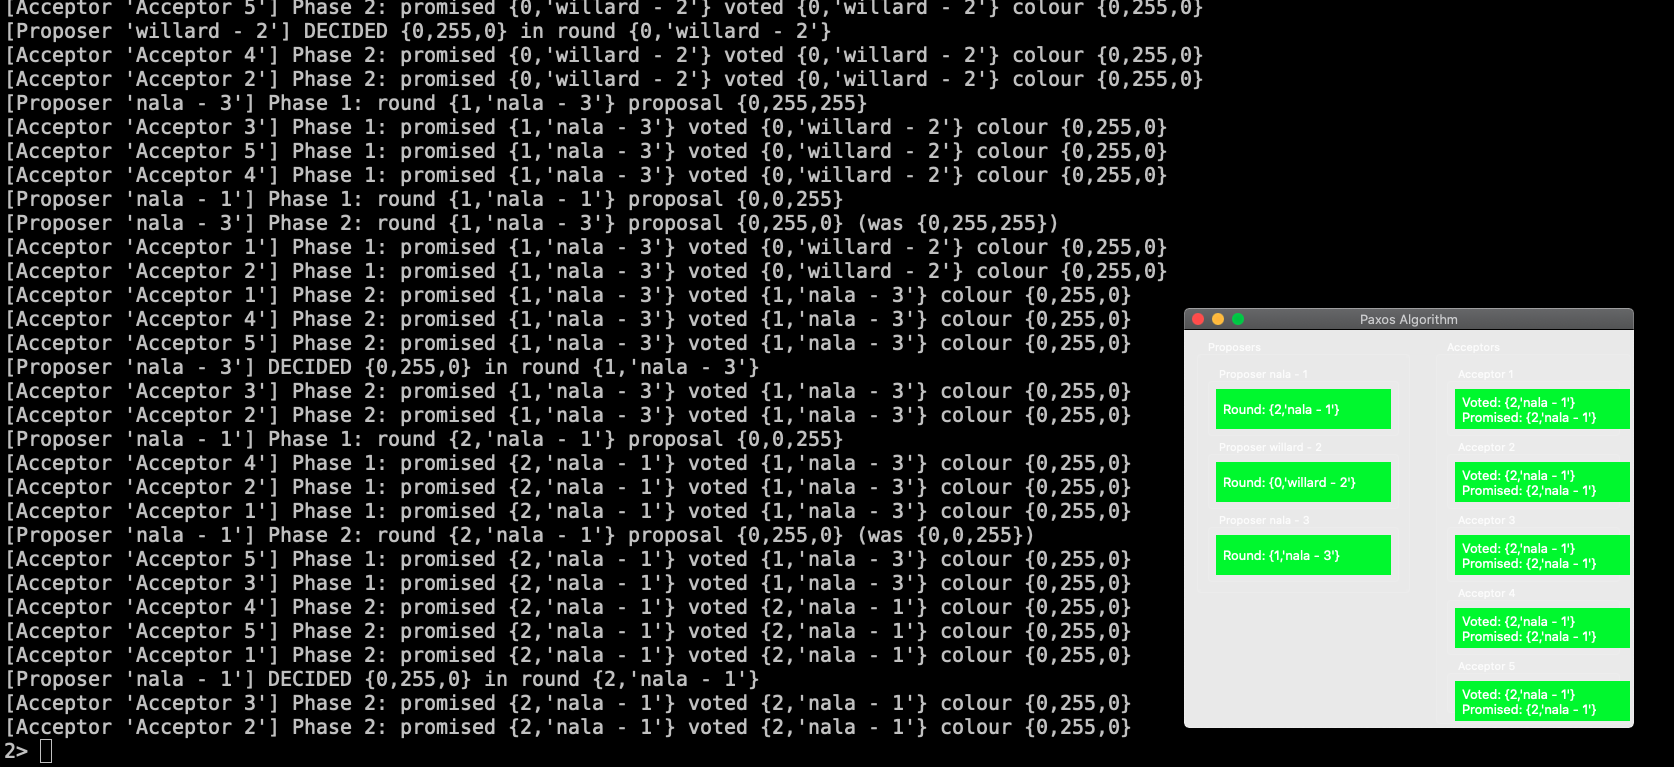
\includegraphics[width=\textwidth]{delay200ms}
    \captionof{figure}{Acceptors with a delay of 200 ms}
\end{minipage}
\item Test with 1000ms Delay, finishes successfully \lstinline|paxy:start(local,{1000,na},[1,1,1]).|\\\\
\begin{minipage}[t]{\linewidth}
    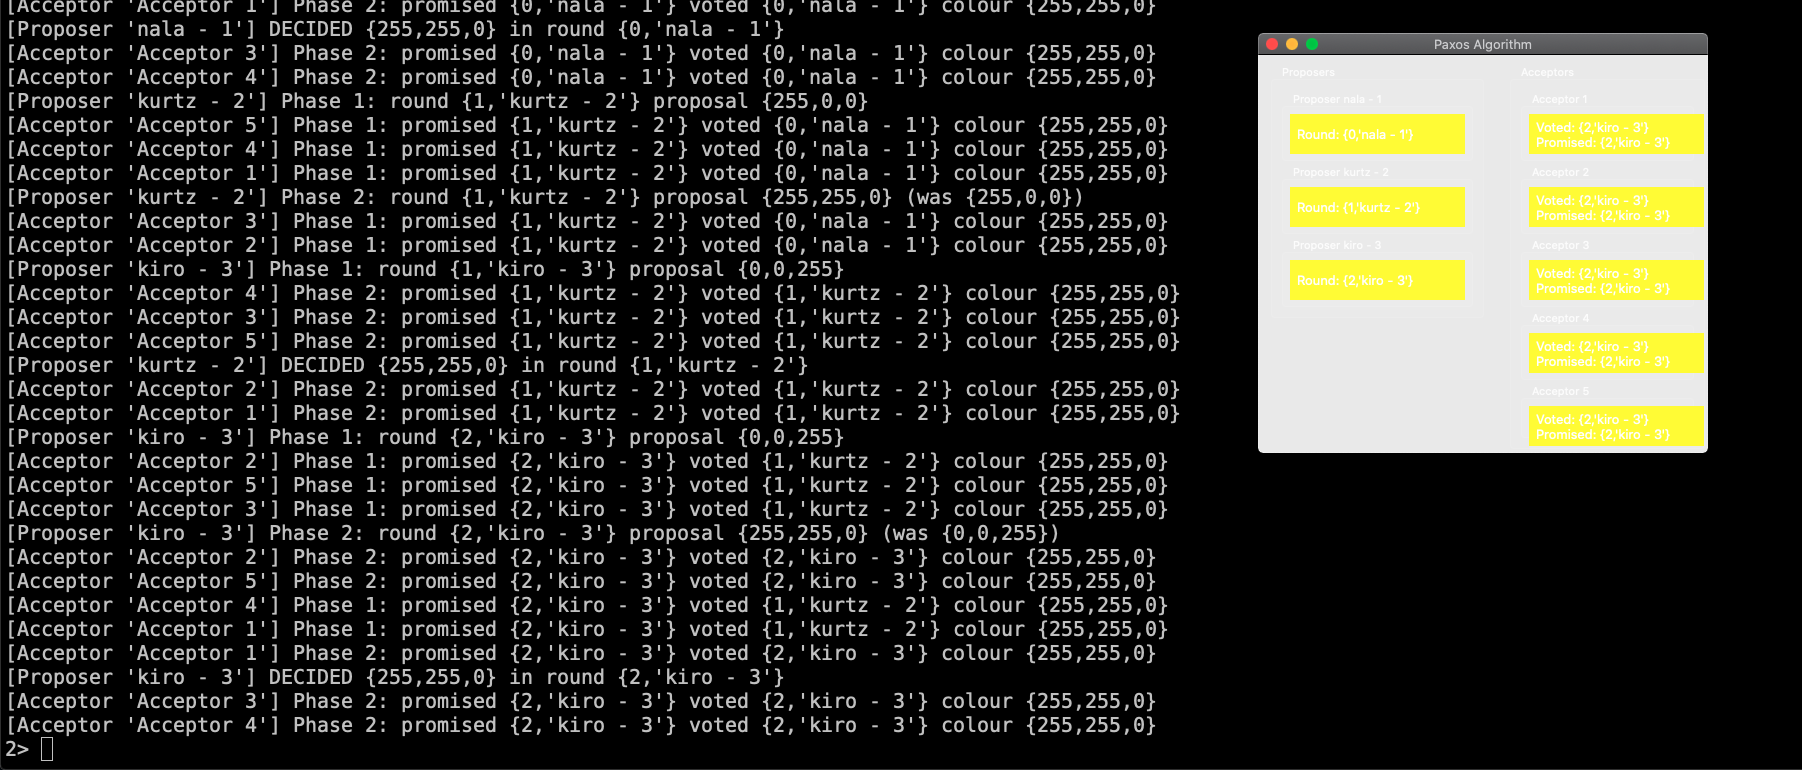
\includegraphics[width=\textwidth]{delay1000ms}
    \captionof{figure}{Acceptors with a delay of 1000 ms}
\end{minipage}
\item Test with 3000ms Delay, finishes successfully \lstinline|paxy:start(local,{3000,na},[1,1,1]).|\\\\
\begin{minipage}[t]{\linewidth}
    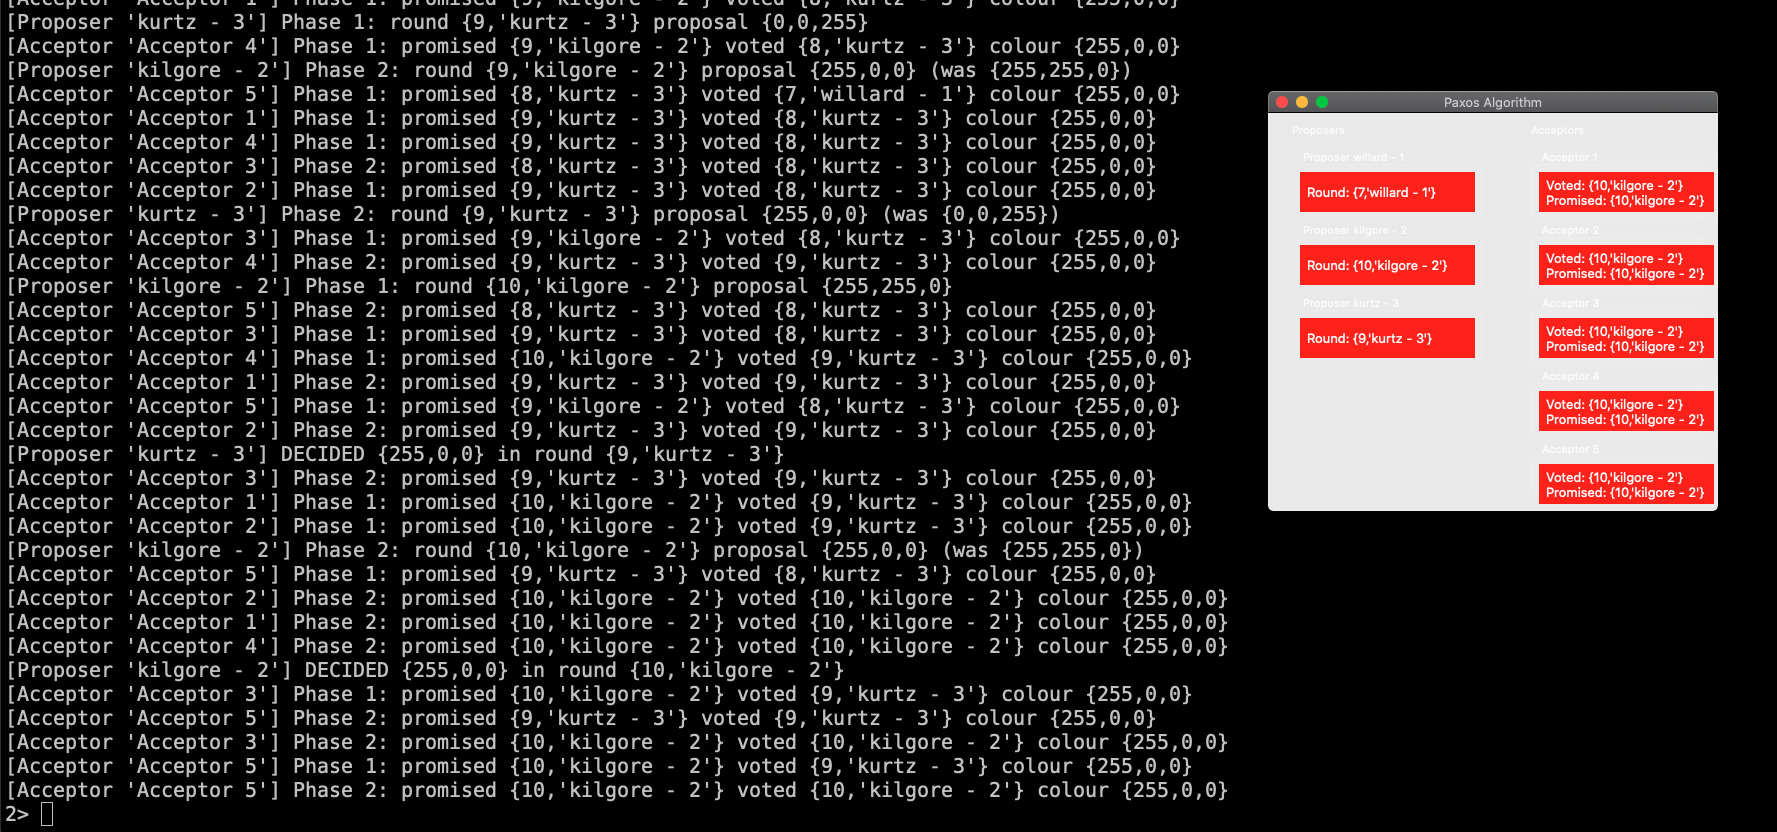
\includegraphics[width=\textwidth]{delay3000ms}
    \captionof{figure}{Acceptors with a delay of 3000 ms}
\end{minipage}
\item Test with 5000ms Delay, \color{red}{No Consensus reached} \lstinline|paxy:start(local,{5000,na},[1,1,1]).|\\\\
  \begin{minipage}[t]{\linewidth}
    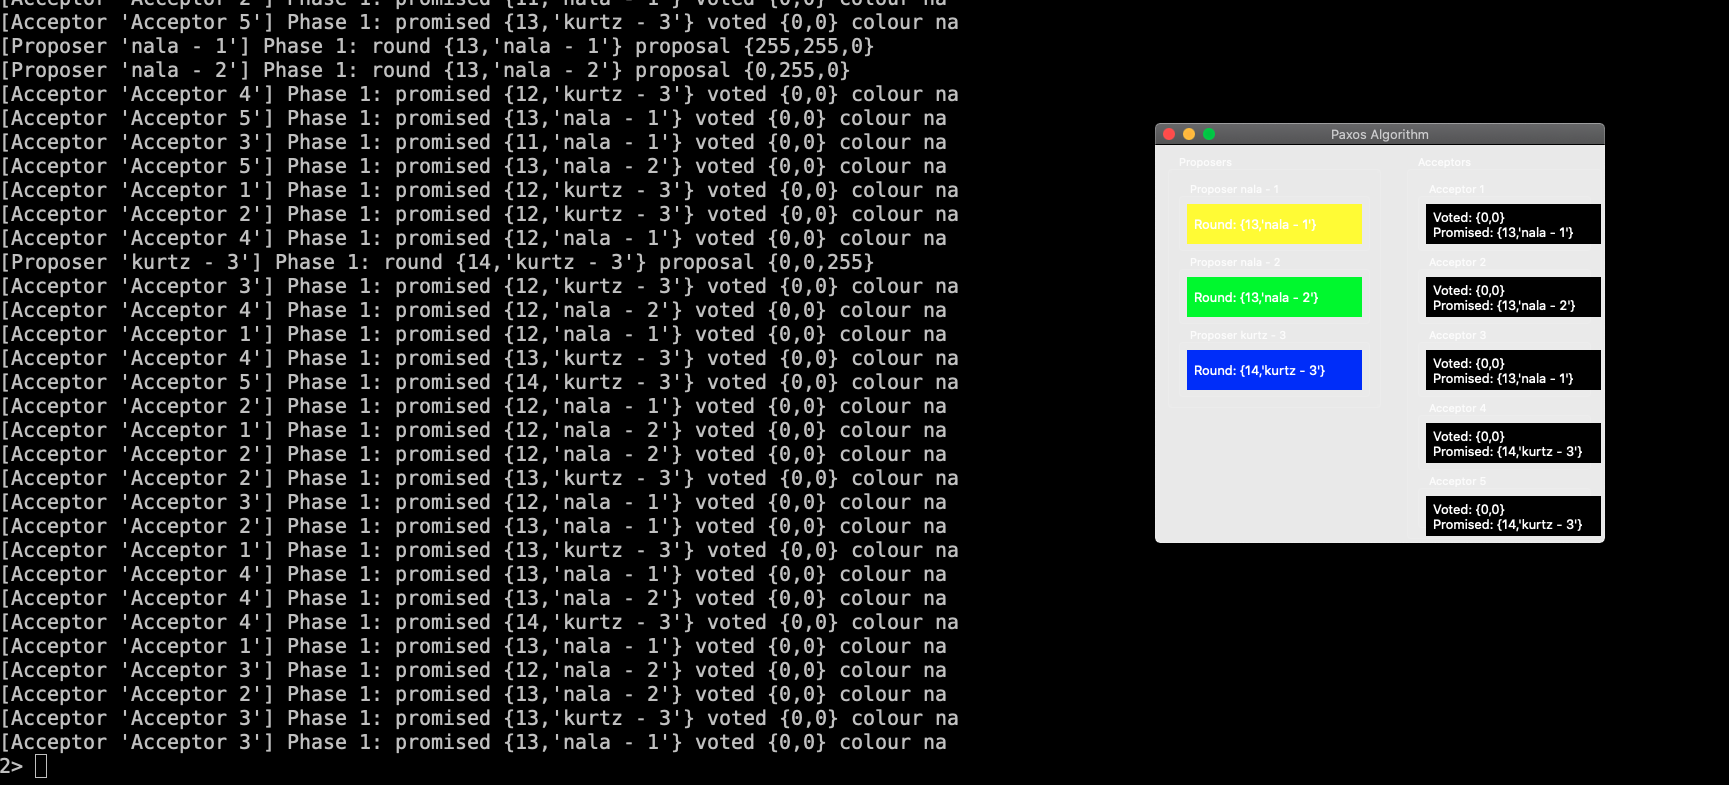
\includegraphics[width=\textwidth]{delay5000ms}
    \captionof{figure}{Acceptors with a delay of 5000 ms}
  \end{minipage}\\\\\\\\\\
\item Table with Time Results\\\\
  \begin{table}[h!]
  \begin{tabular}{ |c|c|c|c|c|  }
    \hline
    \multicolumn{5}{|c|}{Running Time} \\
    \hline
    Experiment & User Time & System Time & CPU Percentage & Total\\
    \hline
    Delay 200ms & 1.10s & 0.26s & 4\% & 28.779\\
    Delay 1000ms & 1.33s & 0.31s & 8\% & 30.468\\
    \textbf{Delay 3000ms} & 2.45s & 0.59s & 4\% & 1:14.90\\
    \color{red}\textbf{Delay 5000ms - No consensus} & 2.82s & 0.75s & 0\% & 8:10.46\\
    \hline
  \end{tabular}
  \captionof{figure}{Different Running times from Linux terminal changing Delay configuration of Acceptors messages}
  \label{table:acceptorsDelay}
  \end{table}
\end{itemize}
After trying different values for the \textbf{delay}, we have found that the
algorithm tries to reach the consensus, according to what we can see on the
\ref{table:acceptorsDelay} table. However, with a delay of $5000
ms$, the consensus is very difficult to reach by the participants. It requires so
many more rounds, and taking into consideration that the timeout of the
proposers is much more less than the acceptors, that round is ignored because the proposer will be waiting for the following round.
\\\\
Saying this, we believe that there should be an $N$ in milliseconds where the
algorithm does not terminate because all the rounds are abandoned by the proposers, producing an Starvation of the consensus.

\subsubsection{Avoid Sorry messages}
\textbf{\large{Question}}\\\\
Avoid sending sorry messages by commenting the corresponding sentences in the
acceptor. Q) Could you even come to an agreement when sorry messages are not
sent?
\\\\
\textbf{\large{Answer}}\\\\
Yes, it can come to an agreement without sorry messages because those messages
are not affecting the behaviour neither on the \textbf{collect} nor in \textbf{vote} functions.
\\\\
\subsubsection{Dropping Messages}
\textbf{\large{Question}}\\\\
Try randomly dropping promise and/or vote messages in the acceptor. If you drop
too many messages a quorum will of course never be found, but we could probably
lose quite many. Q) What percentage of messages can we drop until consensus is
not longer possible?
\\\\
\textbf{\large{Answer}}\\\\
\begin{itemize}
\item Test with 10\% Dropping messages, finishes successfully \lstinline|paxy:start(local,{na,1},[1,1,1]).|\\\\
\begin{minipage}[t]{\linewidth}
    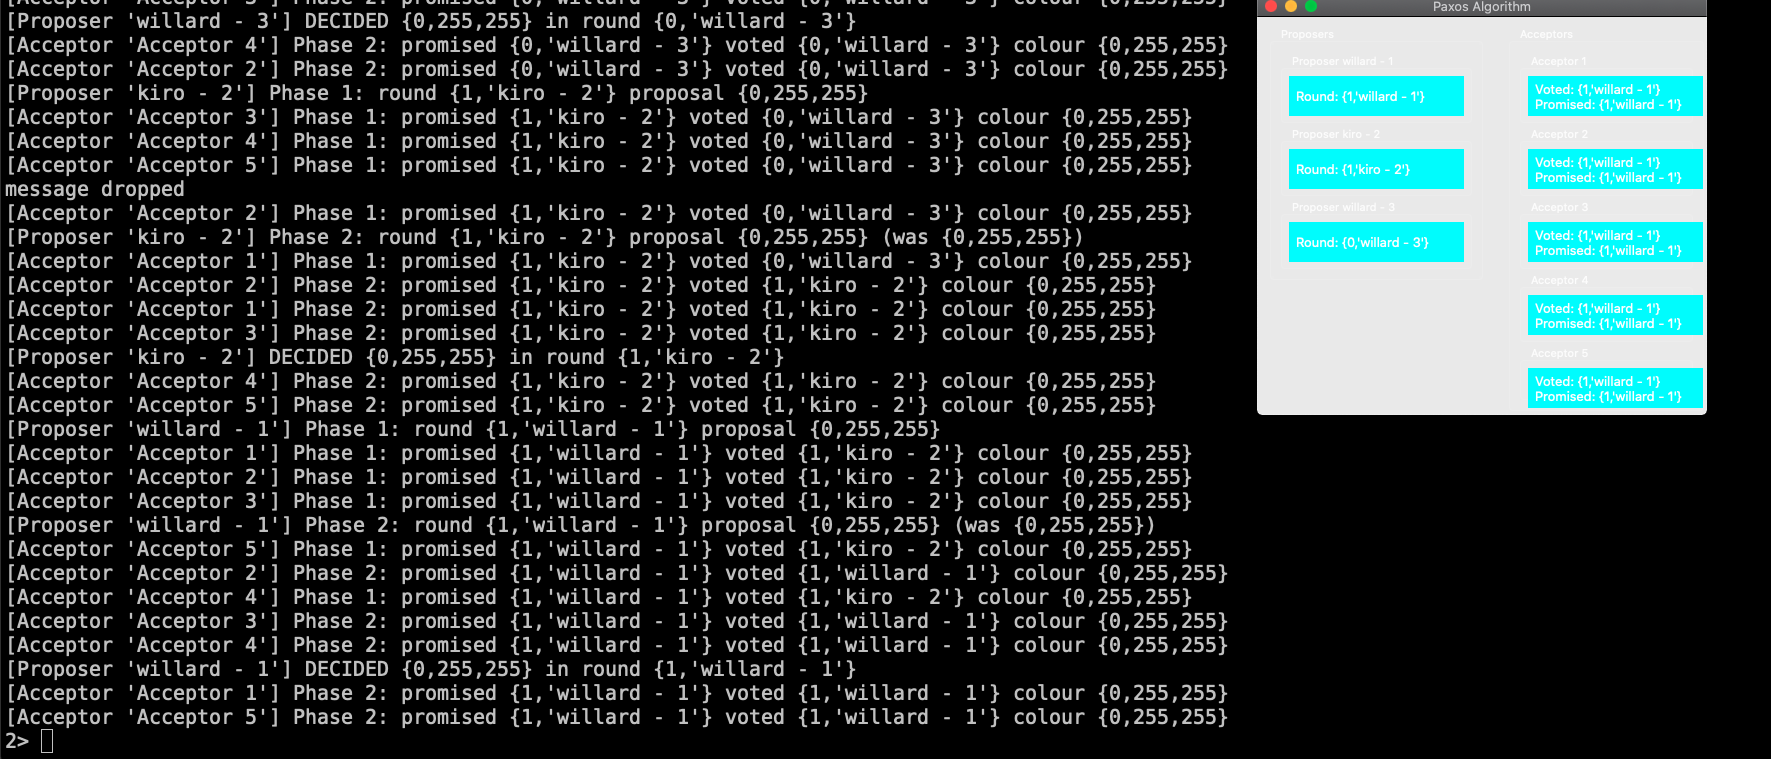
\includegraphics[width=\textwidth]{drop1}
    \captionof{figure}{Acceptors with 10\% dropping messages}
\end{minipage}
\item Test with 30\% Dropping messages, finishes successfully \lstinline|paxy:start(local,{na,3},[1,1,1]).|\\\\
  \begin{minipage}[t]{\linewidth}
    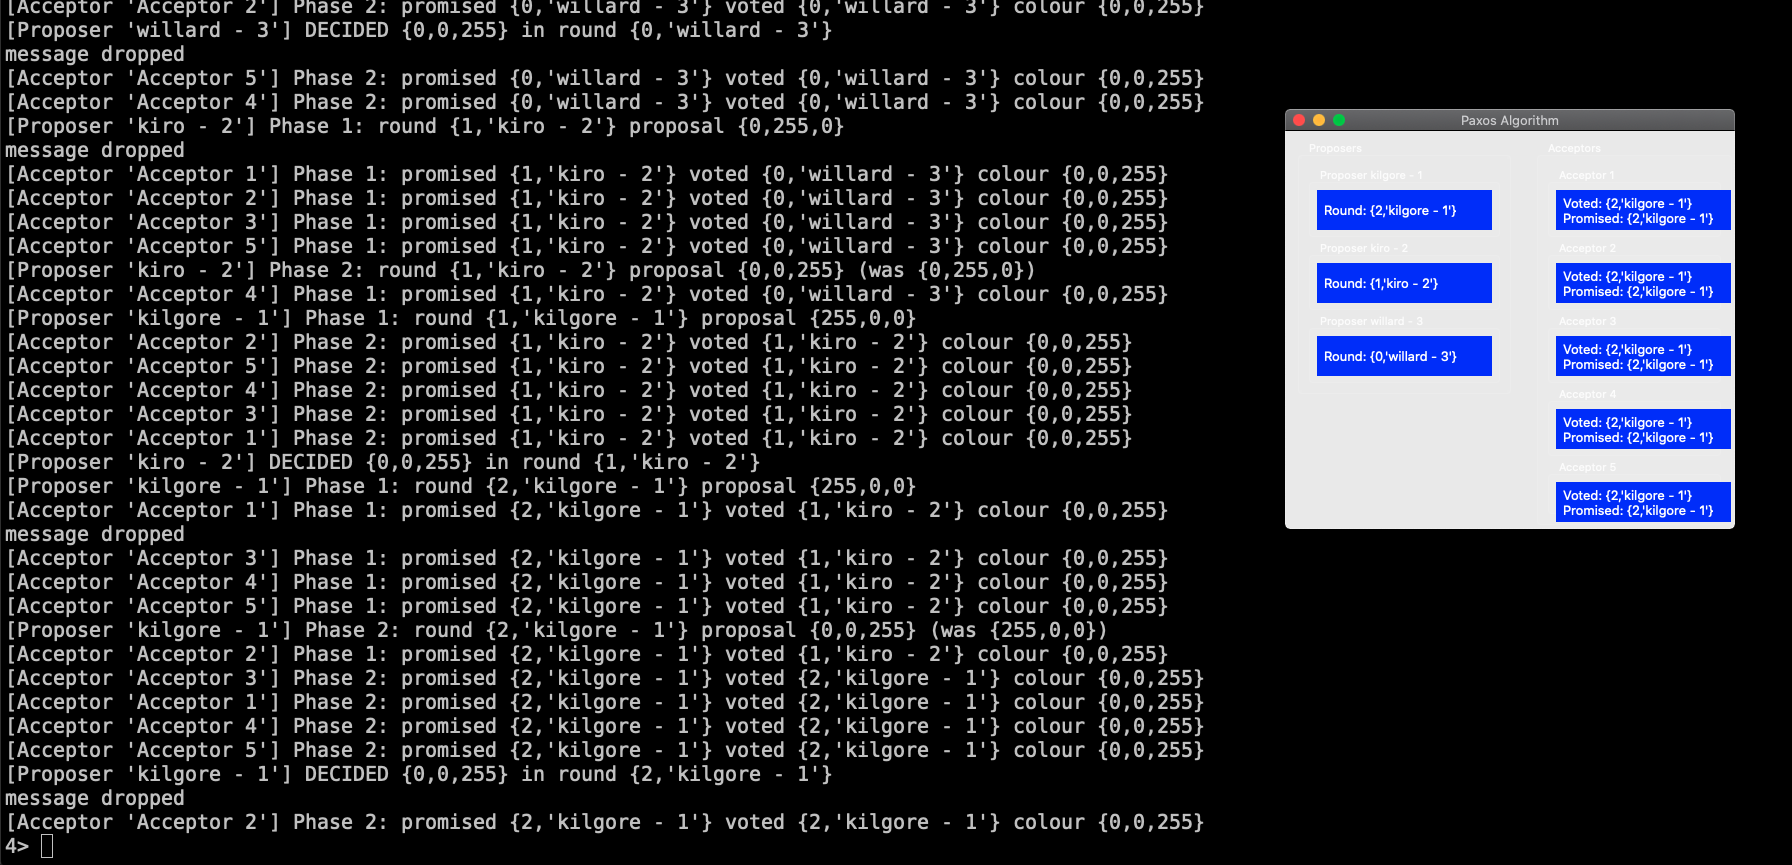
\includegraphics[width=\textwidth]{drop3}
    \captionof{figure}{Acceptors with 30\% dropping messages}
\end{minipage}
\item Test with 50\% Dropping messages, finishes successfully \lstinline|paxy:start(local,{na,5},[1,1,1]).|\\\\
  \begin{minipage}[t]{\linewidth}
    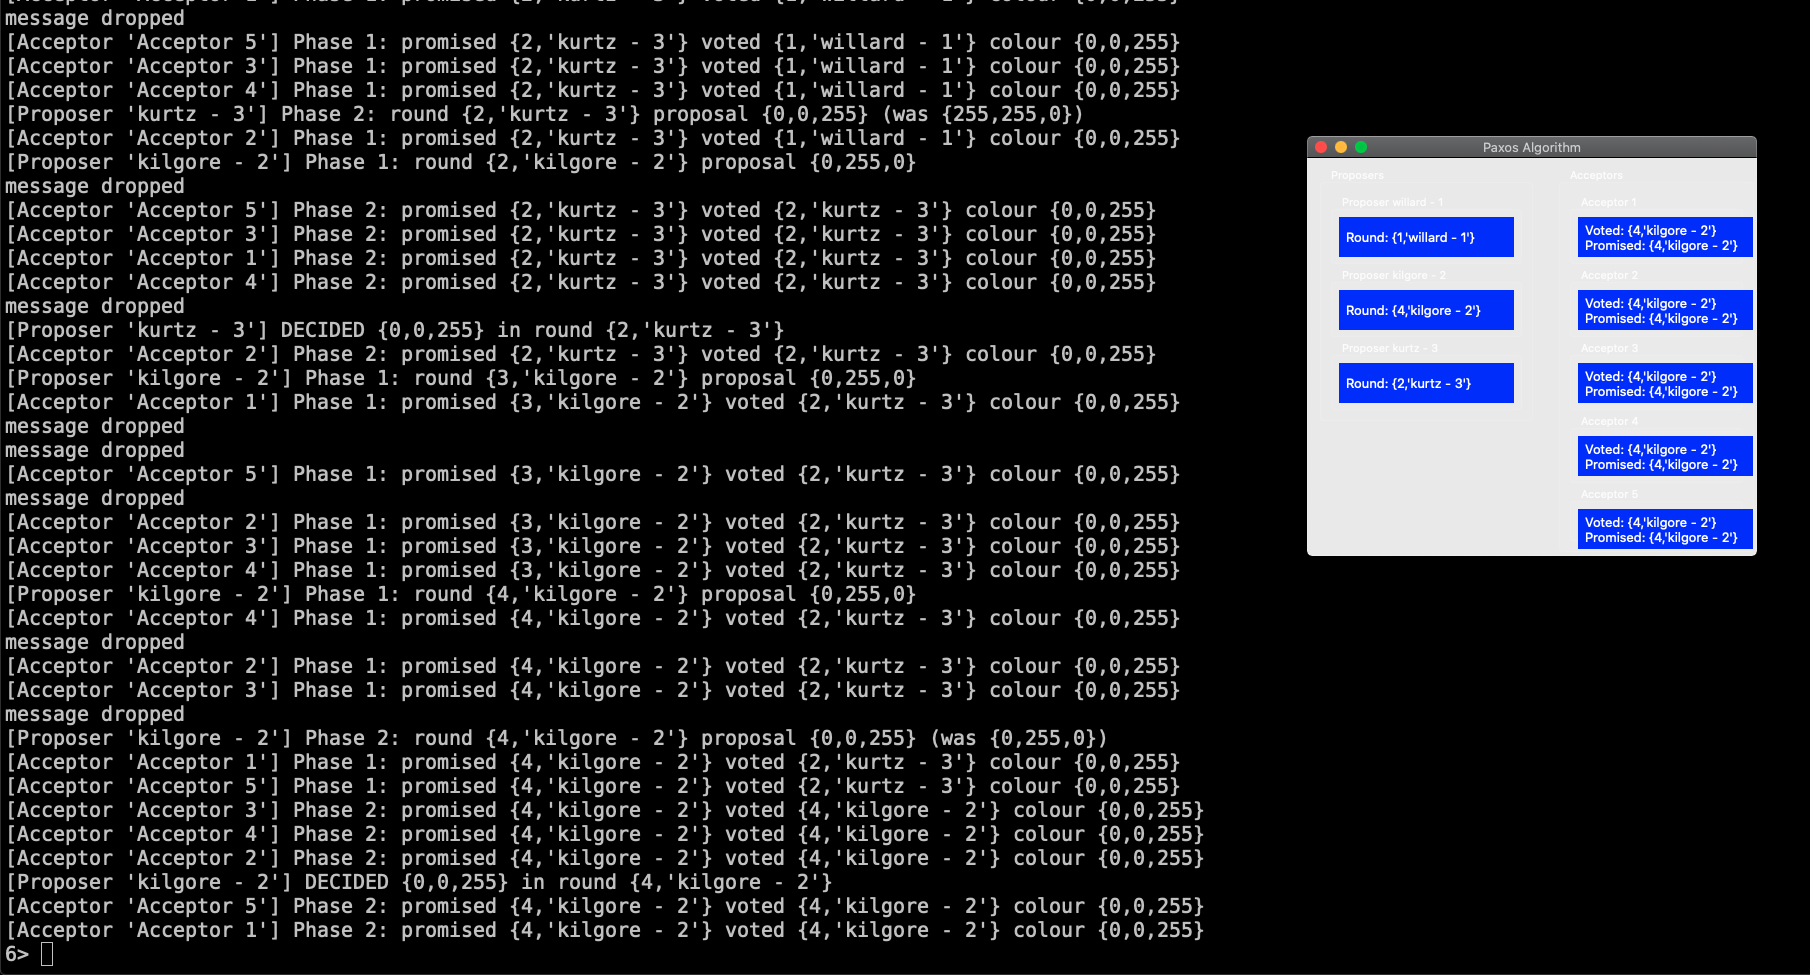
\includegraphics[width=\textwidth]{drop5}
    \captionof{figure}{Acceptors with 50\% dropping messages}
  \end{minipage}
\item Test with 60\% Dropping messages, \color{red}{No consensus reached} \lstinline|paxy:start(local,{na,6},[1,1,1]).|\\\\
  \begin{minipage}[t]{\linewidth}
    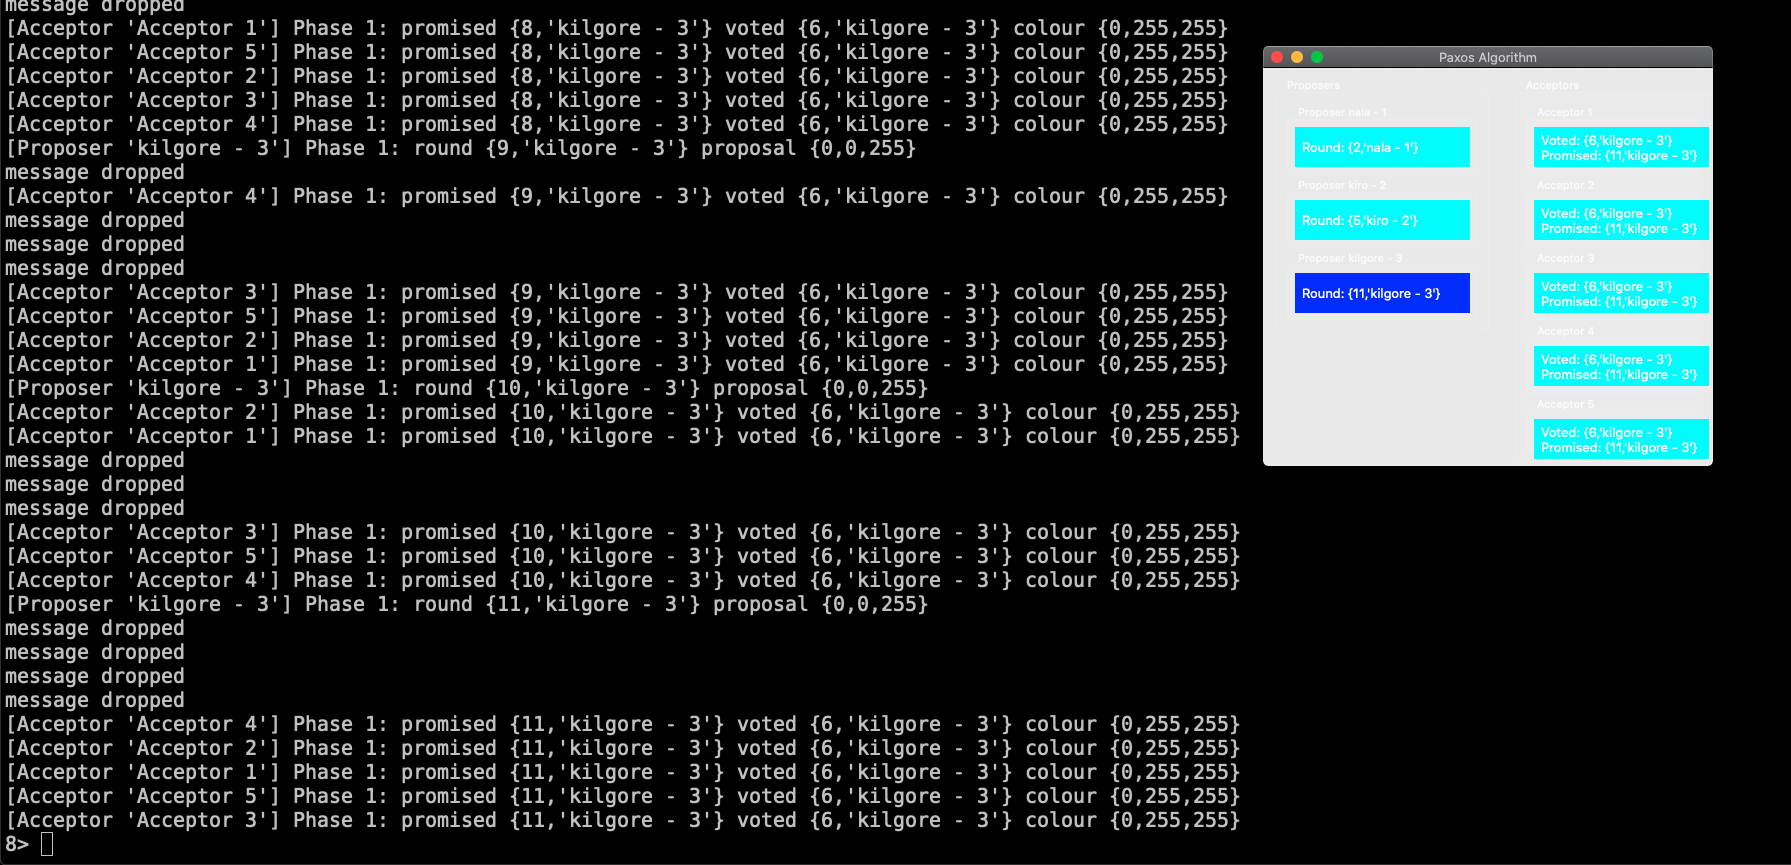
\includegraphics[width=\textwidth]{drop6}
    \captionof{figure}{Acceptors with 60\% dropping messages}
  \end{minipage}
\end{itemize}
The percentage of messages that we need to drop until consensus is not longer
possible is $60\%$. This can be explained because proposers need a Quorum of $50\%
+ 1$ of the acceptors and we are dropping more then half of the messages. Since the probability of dropping a message is uniformly random distributed, when the \textbf{number} of dropping messages is \textbf{increased}, the Probability of reaching a Quorum decreases proportionally, with a big dive after $60\%$.
\\\\
     
\subsubsection{Dynamic Number of Acceptors and Proposers}
\textbf{\large{Question}}\\\\
Try increasing the number of acceptors and proposers. Q) What is the impact of having more acceptors while keeping the same number of proposers? What if we have more proposers while keeping the same number of acceptors?
\\\\
\textbf{\large{Answer}}\\\\
Increasing the number of acceptors will slightly increase the time that the algorithm
needs to reach the consensus because it will increment the number of messages received in the collect procedure and the messages sent from the Proposers to the Acceptors.
\\\\
\begin{minipage}[t]{\linewidth}
    \centering
    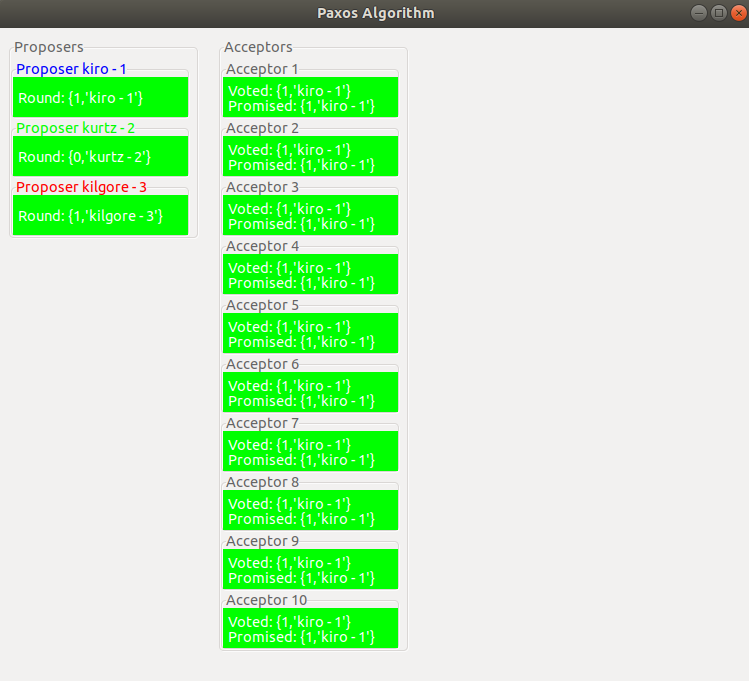
\includegraphics[width=0.5\textwidth]{10Acceptors}
    \captionof{figure}{Running 3 Proposers and 10 Acceptors}
\end{minipage}\\\\
Regarding increasing the amount of Proposers but keeping the number of
Acceptors, we have realized that it took more time to reach the consensus since the number of colors also increases. Thus, the initial conditions are less favorable to reach a consensus. Furthermore, the number of Proposers that have lost the ballot in each round need to wait for the most Voted Value, and therefore reach the final consensus. Said that, more rounds are needed and each execution is slower.\\\\
\begin{minipage}[t]{\linewidth}
  \centering
   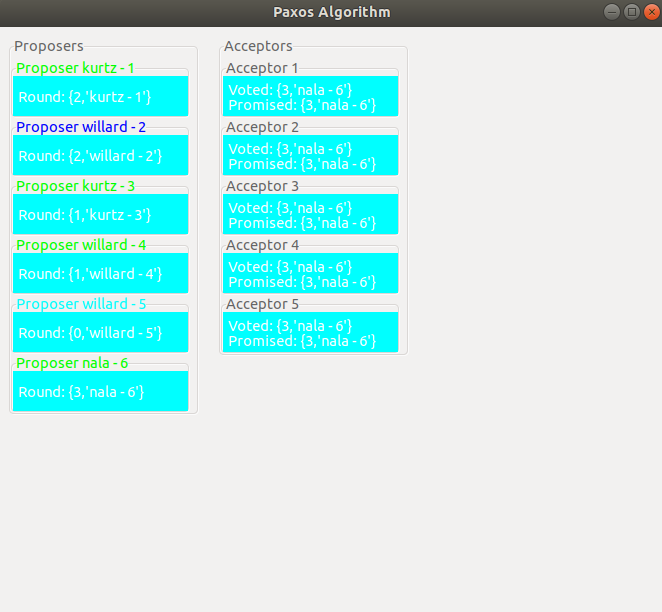
\includegraphics[width=0.5\textwidth]{6Proposers}
   \captionof{figure}{Running 6 Proposers and 5 Acceptors}
\end{minipage}
\subsubsection{Remote Mode}
\textbf{\large{Question}}\\\\
Adapt the paxy module to create the proposers in a remote Erlang instance (named paxy-pro) and to ensure that they can connect correctly to the acceptors, which must be created in a different remote Erlang instance (named paxy-acc). Note that the acceptors have to use locally registered names. Remember how processes are created remotely, how names registered in remote nodes are referred, and how Erlang runtime should be started to run distributed programs.
\\\\
\textbf{\large{Answer}}\\\\
We have adapted Erlang code in order to run either remote or in local mode.
\\\\
Now \lstinline|paxy:start(...)| function receives 2 parameters, $Mode$ which can
be $local \mid remote$ and the list of $Sleep$ like the older code.
\\\\
In order to run it in \textbf{remote} mode we need to do the following steps:

\begin{itemize}
  \item First Start \textbf{erlang} instance with remote mode for acceptors

\begin{lstlisting}
\$ erl -sname paxy-acc -noshell   
\end{lstlisting}

\item After that we can run the program in remote mode

\begin{lstlisting}
\$ erl -sname paxy-pro -remsh paxy-acc
Eshell V10.5.2  (abort with ^G)

(paxy-acc@My-Machine)1> paxy:start(remote,[1,1,1]).
\end{lstlisting}
      
\end{itemize}

\subsection{Fault tolerance}
\subsubsection{Question}

Simulate a crash and restart of an acceptor using the crash procedure below (to be placed in the paxy module) and check if it recovers successfully (with the right state). You can specify a ’na’ value for the PanelId of the acceptor, as it will get this value from the persistent storage.

\subsubsection{Answer}

We have adapted Erlang code in order to simulate a crash. Although our solution
is configurable there are some symbols that we kept in order to not overload end
user with a lot of information about different configuration parameters.\\\\

Saying this, you can run the solution and in the middle send crash messages, but those messages should relay on \textbf{Acceptors} names.\\\\

Lets give an example. As in the section before we have explained, you need to start first erlang instance for Acceptors in other terminal like this:\\\\

\begin{lstlisting}
\$ erl -sname paxy-acc -noshell   
\end{lstlisting}
After that we can run the program in remote mode, but with some specific
configuration to delay acceptors and proposers in order to give us time to send crash messages\\\\

\begin{lstlisting}
\$ erl -sname paxy-pro -remsh paxy-acc
Eshell V10.5.2  (abort with ^G)
        
(paxy-acc@My-Machine)1> paxy:start(remote,{3000,1},[1000,1000,1000],10,3).
\end{lstlisting}

\begin{minipage}[t]{\linewidth}
  \centering
  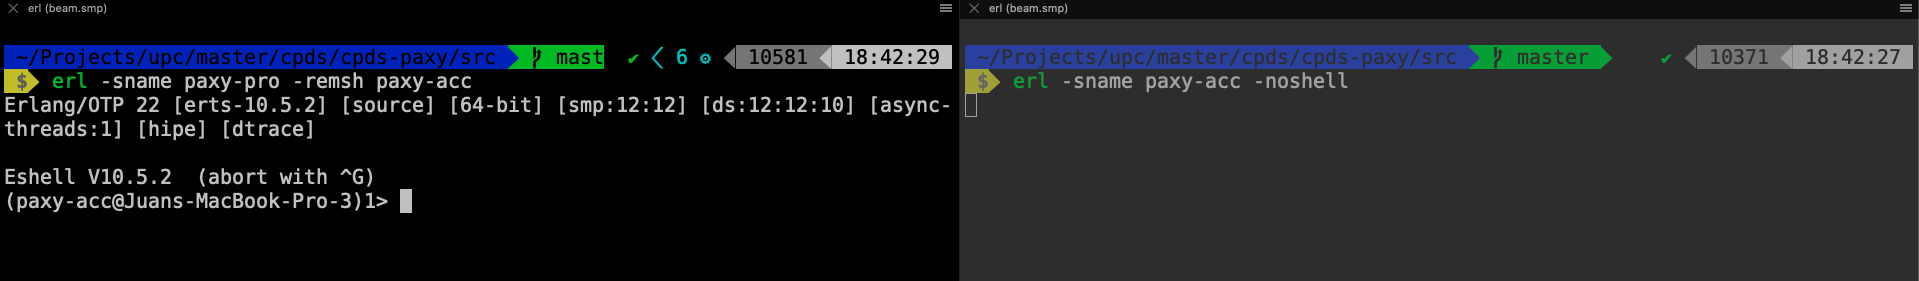
\includegraphics[width=\textwidth]{init_remote}
  \captionof{figure}{Initialize in Remote Mode}
\end{minipage}\\\\

In this example we are starting the solution in remote mode. The second
parameter as it is explained in the code documentation is the \textbf{Acceptor
  Configuration}. It is a Tuple with the following format
\lstinline|{Delay,Drop}| where \textbf{Delay} is the delay in milliseconds that
Acceptors are going to add to send messages, and \textbf{Drop} is the Drop percentage; in this example 10\%.
\\\\
We are going to simulate the first crash on \textbf{Acceptor 3} as we can see in
the following image, with the following message:
\\\\
\begin{lstlisting}
(paxy-acc@My-Machine)1> paxy:crash('Acceptor 3').
\end{lstlisting}

\begin{minipage}[t]{\linewidth}
  \centering
  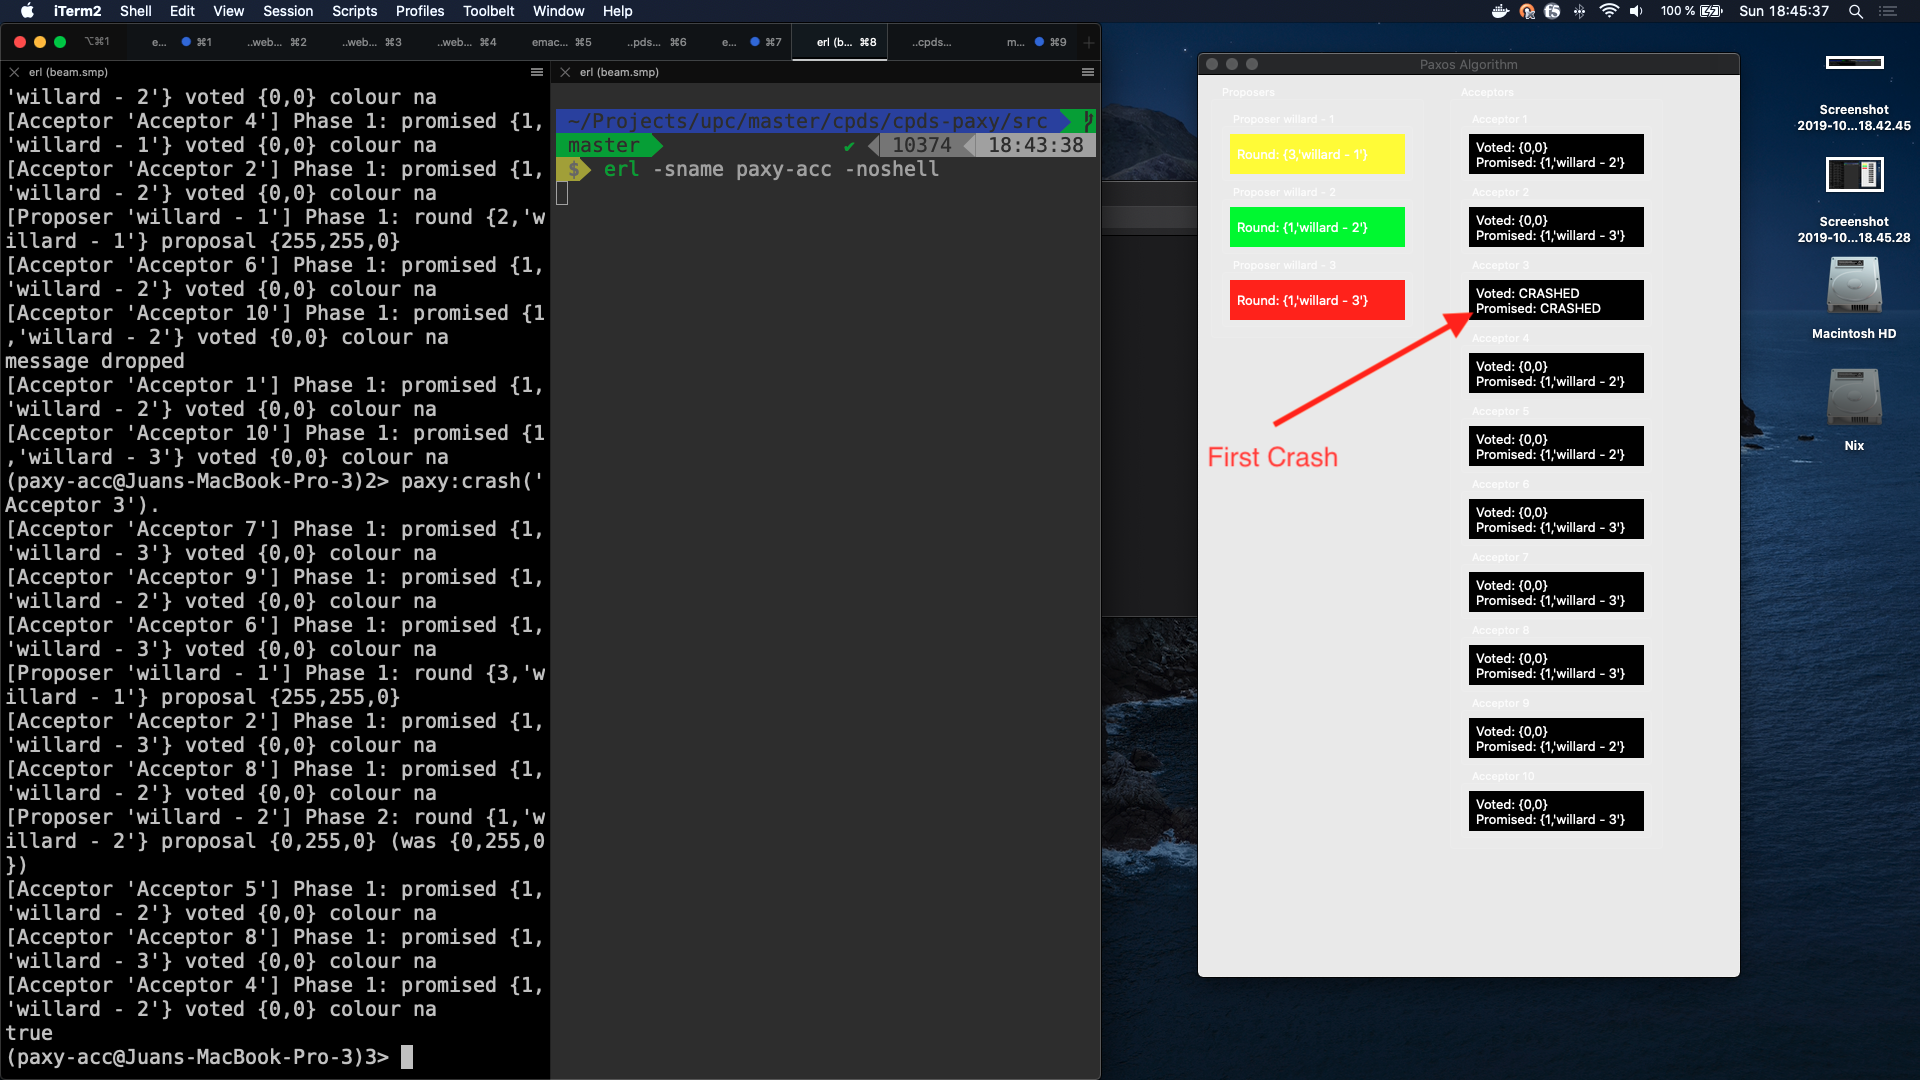
\includegraphics[width=\textwidth]{1crash_acc3}
  \captionof{figure}{Crashing Acceptor 3}
\end{minipage}\\\\

In this example we are crashing \textbf{Acceptor 3}, therefore we are going to
wait it recovered to see everything is working fine as we can see in the image
below:\\\\

\begin{minipage}[t]{\linewidth}
  \centering
  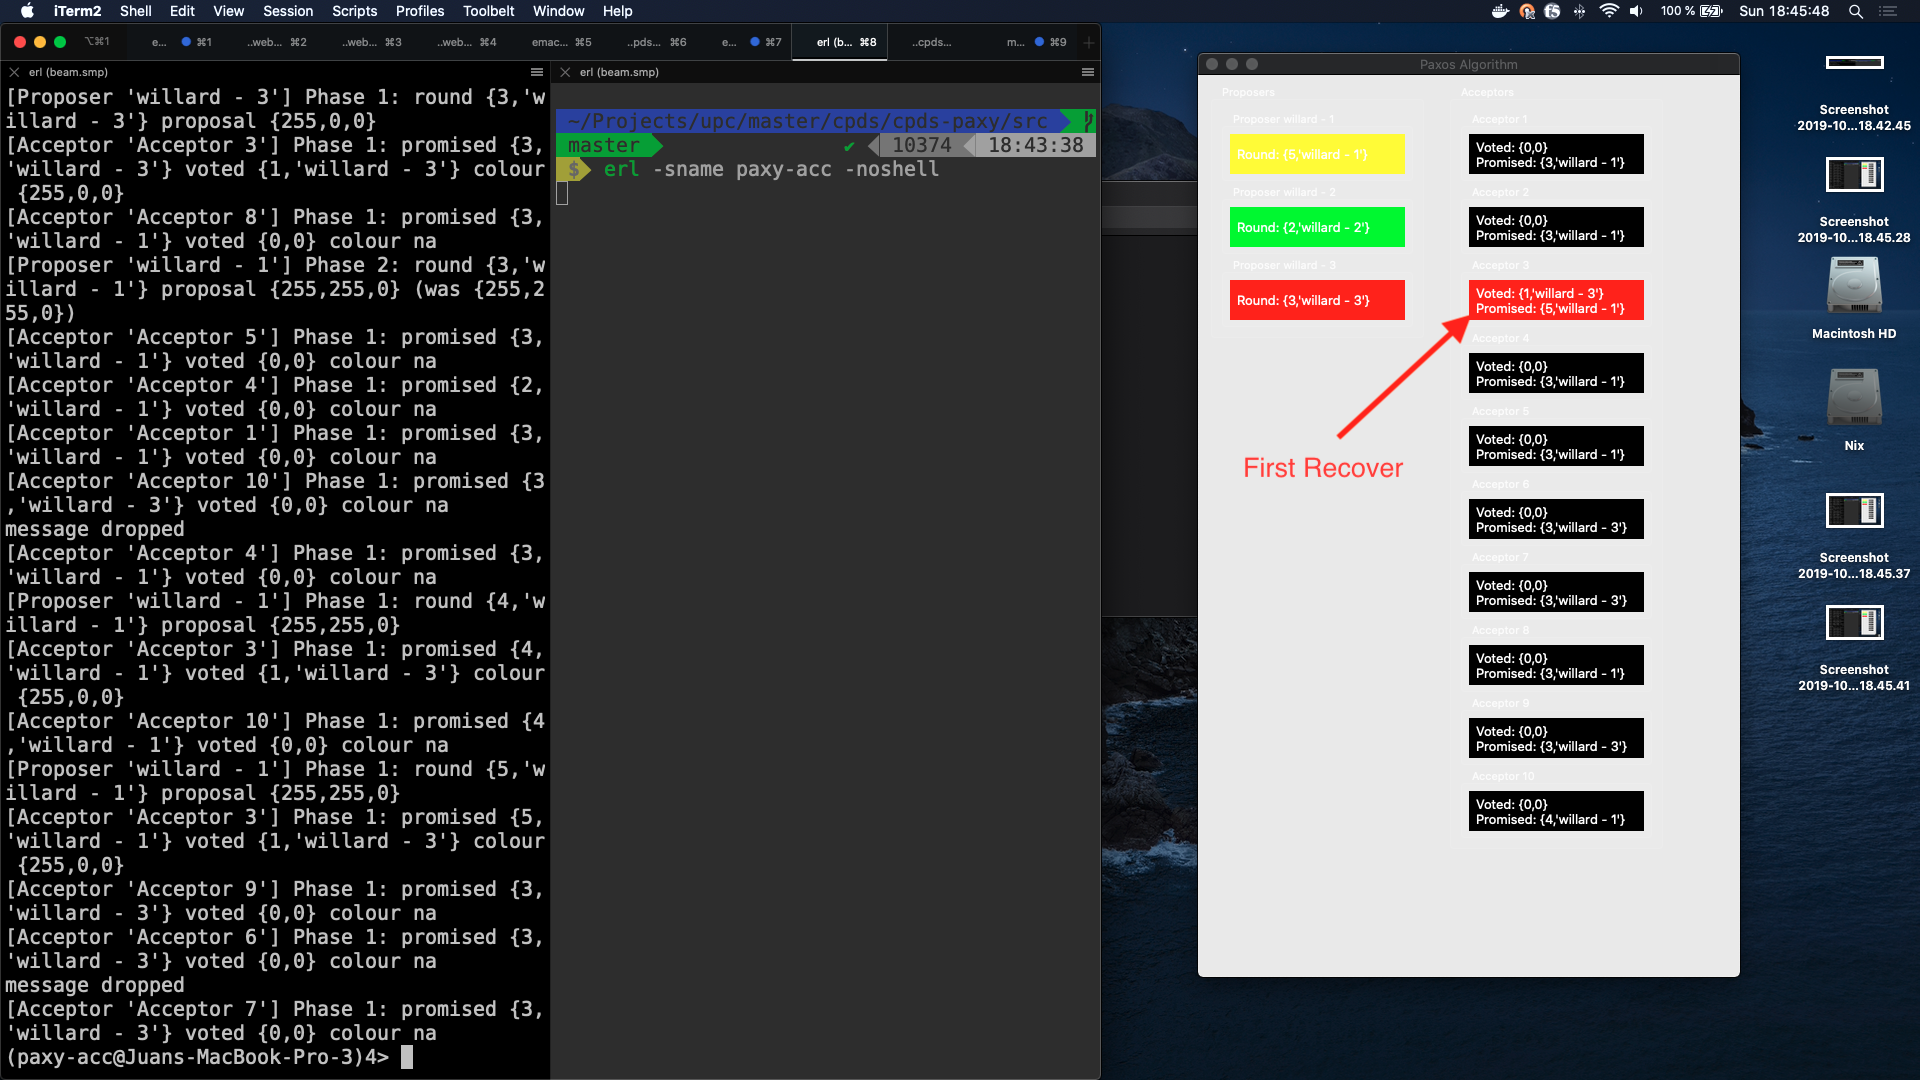
\includegraphics[width=\textwidth]{1recover_acc3}
  \captionof{figure}{Crashing Acceptor 3}
\end{minipage}\\\\

After this, we can crash again the same Acceptor to see now that is with
\textbf{Red} color is going to recover its state again. Lets crash it and wait
for recovering:\\\\

\begin{minipage}[t]{\linewidth}
  \centering
  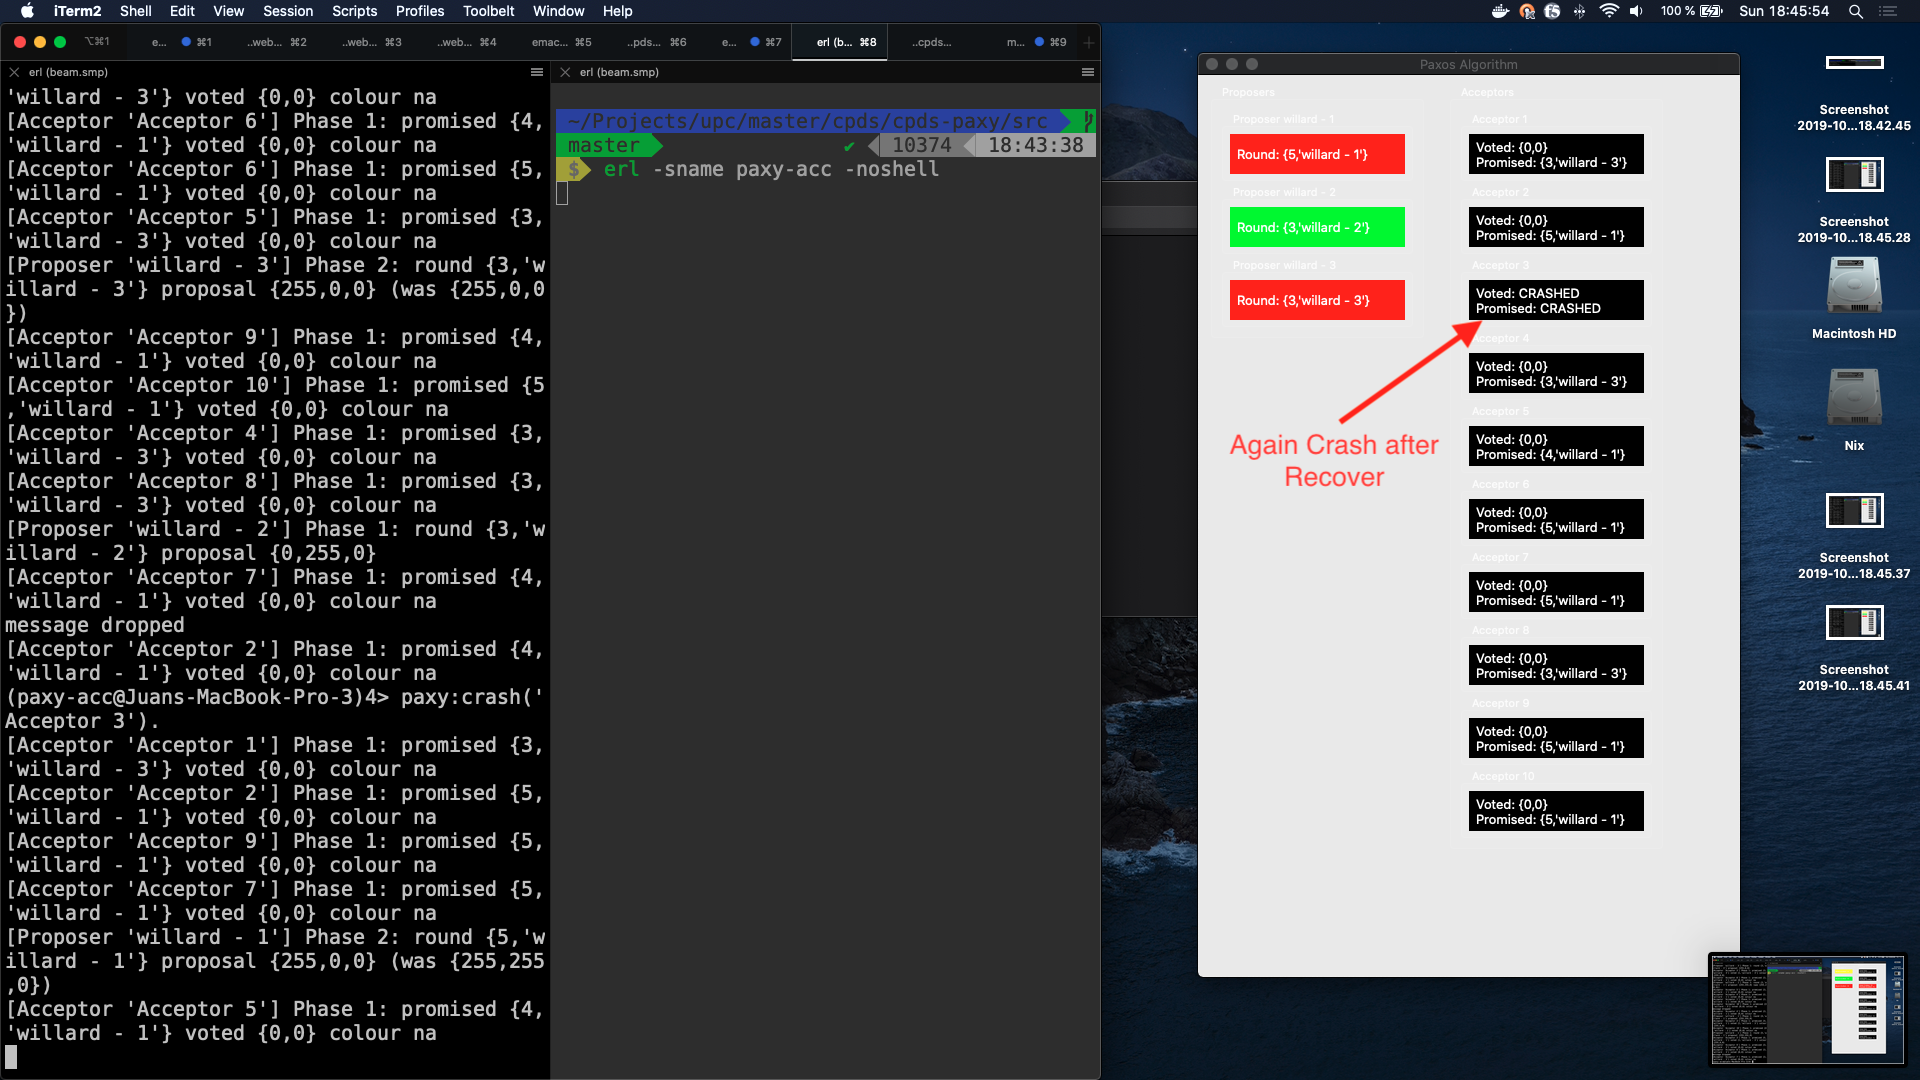
\includegraphics[width=\textwidth]{2crash_acc3}
  \captionof{figure}{Crashing Acceptor 3 - Second Time}
\end{minipage}\\\\

\begin{minipage}[t]{\linewidth}
  \centering
  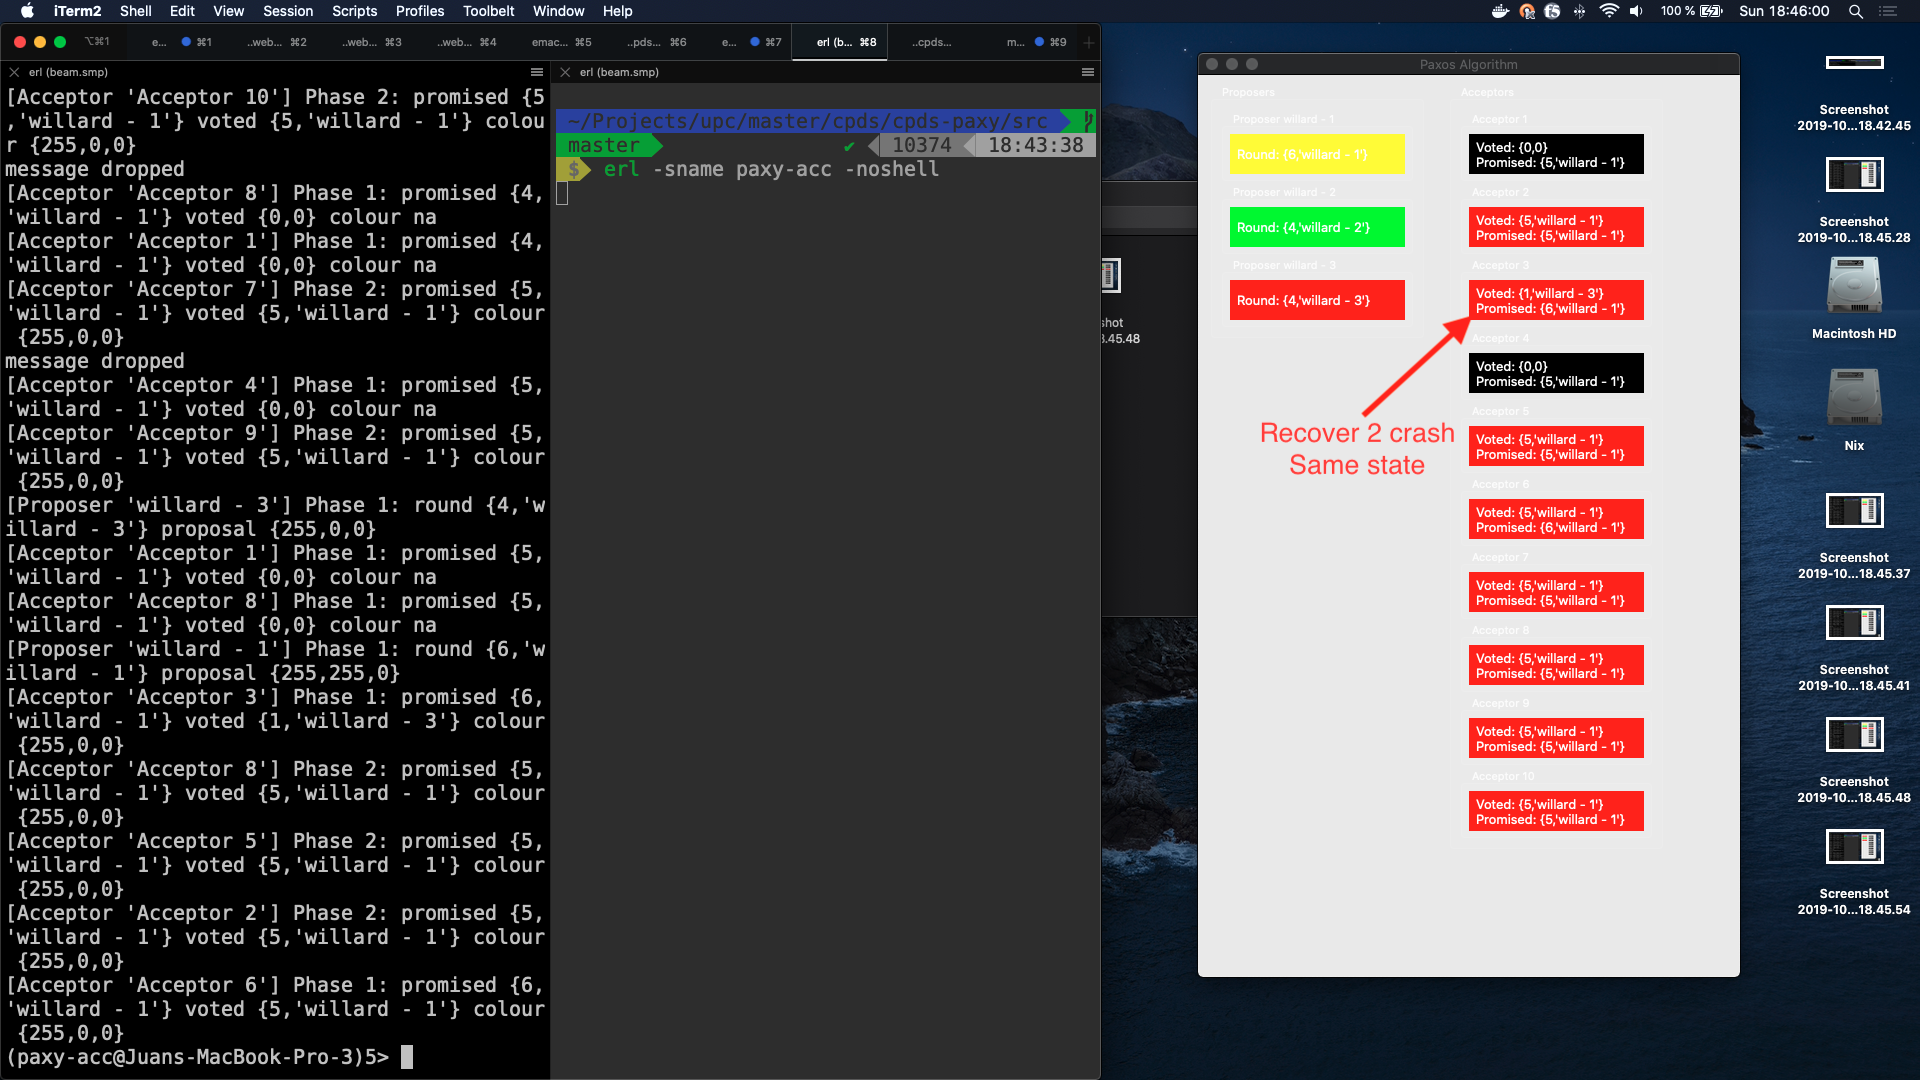
\includegraphics[width=\textwidth]{2recover_acc3}
  \captionof{figure}{Recovering Acceptor 3 - Second Time}
\end{minipage}\\\\

As we can appreciate from the images everything is working as expected.\\\\
Lets try with another Acceptor, lets says \textbf{Acceptor 7} to check that any
Acceptor can be recovered.\\\\

\begin{minipage}[t]{\linewidth}
  \centering
  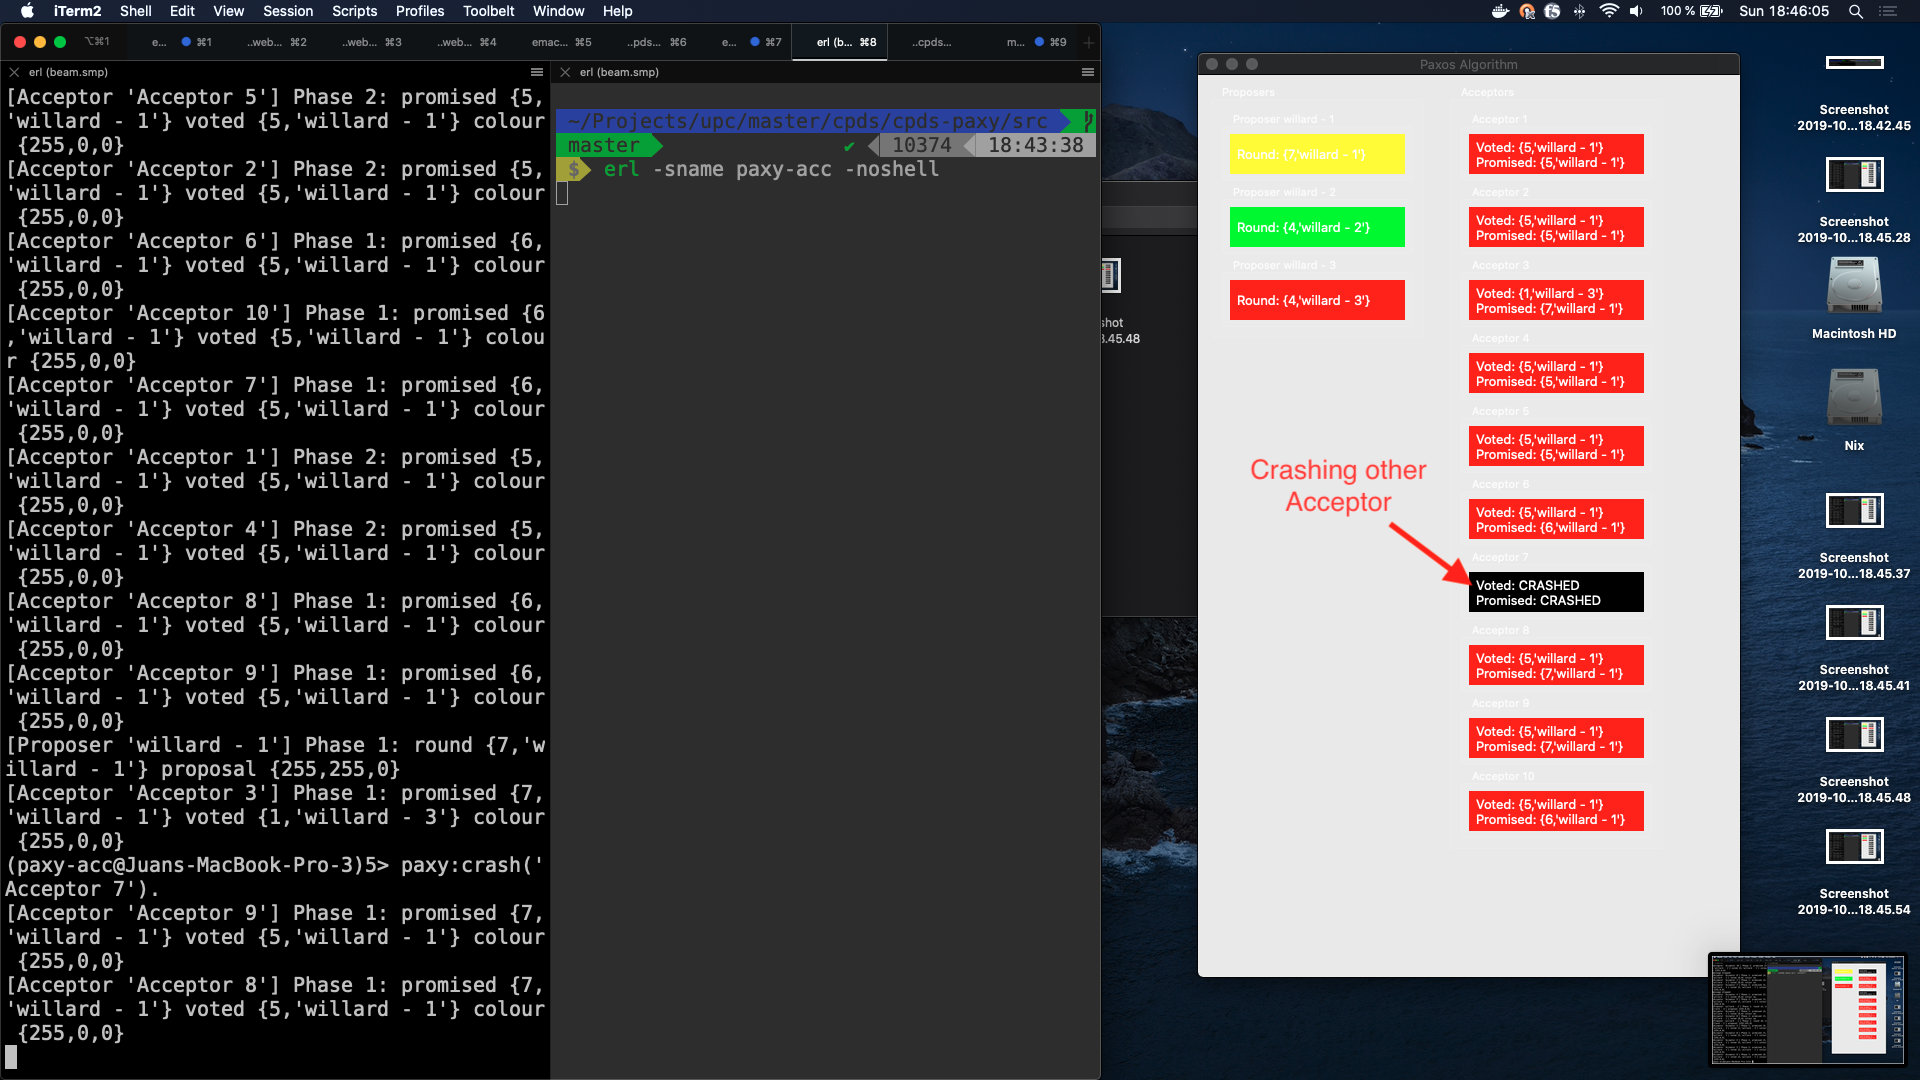
\includegraphics[width=\textwidth]{other_crash}
  \captionof{figure}{Crashing Acceptor 7}
\end{minipage}\\\\

\begin{minipage}[t]{\linewidth}
  \centering
  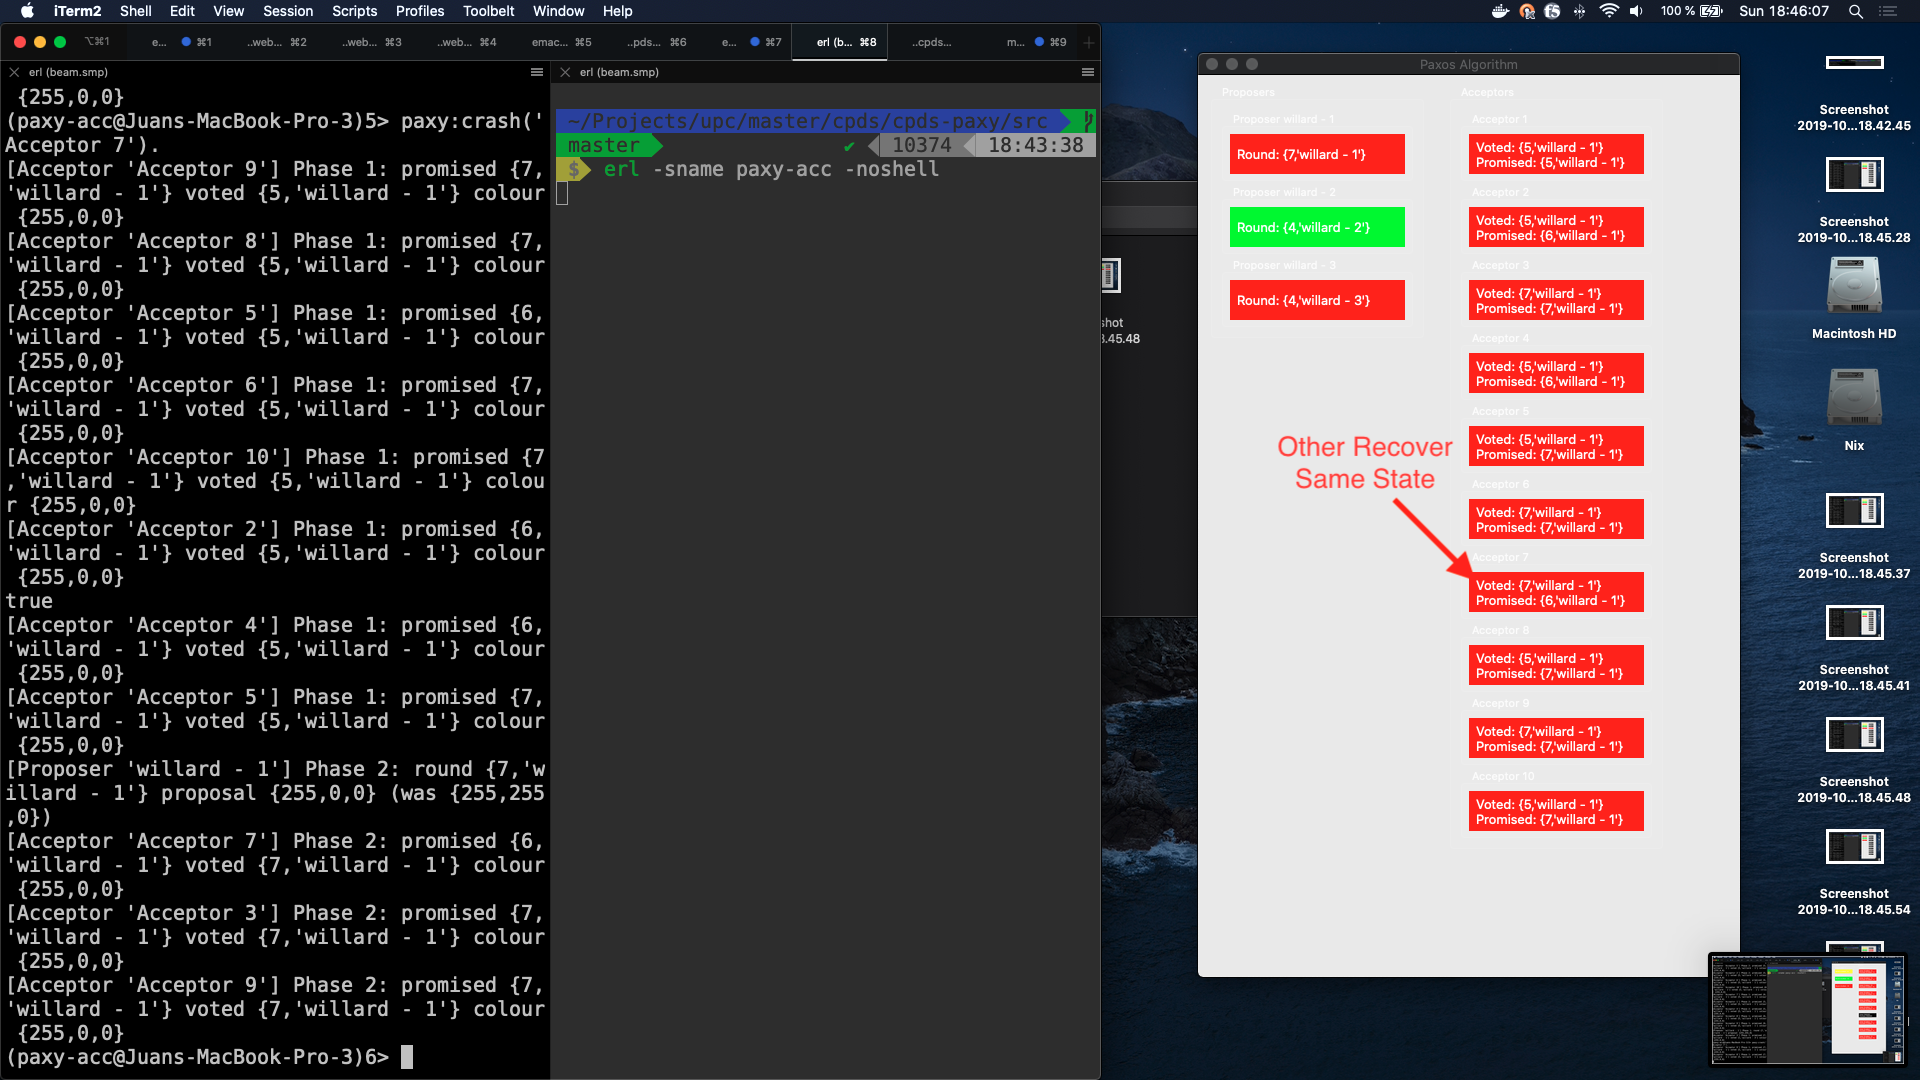
\includegraphics[width=\textwidth]{other_recover}
  \captionof{figure}{Recovering Acceptor 7}
\end{minipage}\\\\

Again everything is working as Expected, and as we can see in the following
image after crashing different Acceptors and waiting for recovering protocol
reach consensus.\\\\

\begin{minipage}[t]{\linewidth}
  \centering
  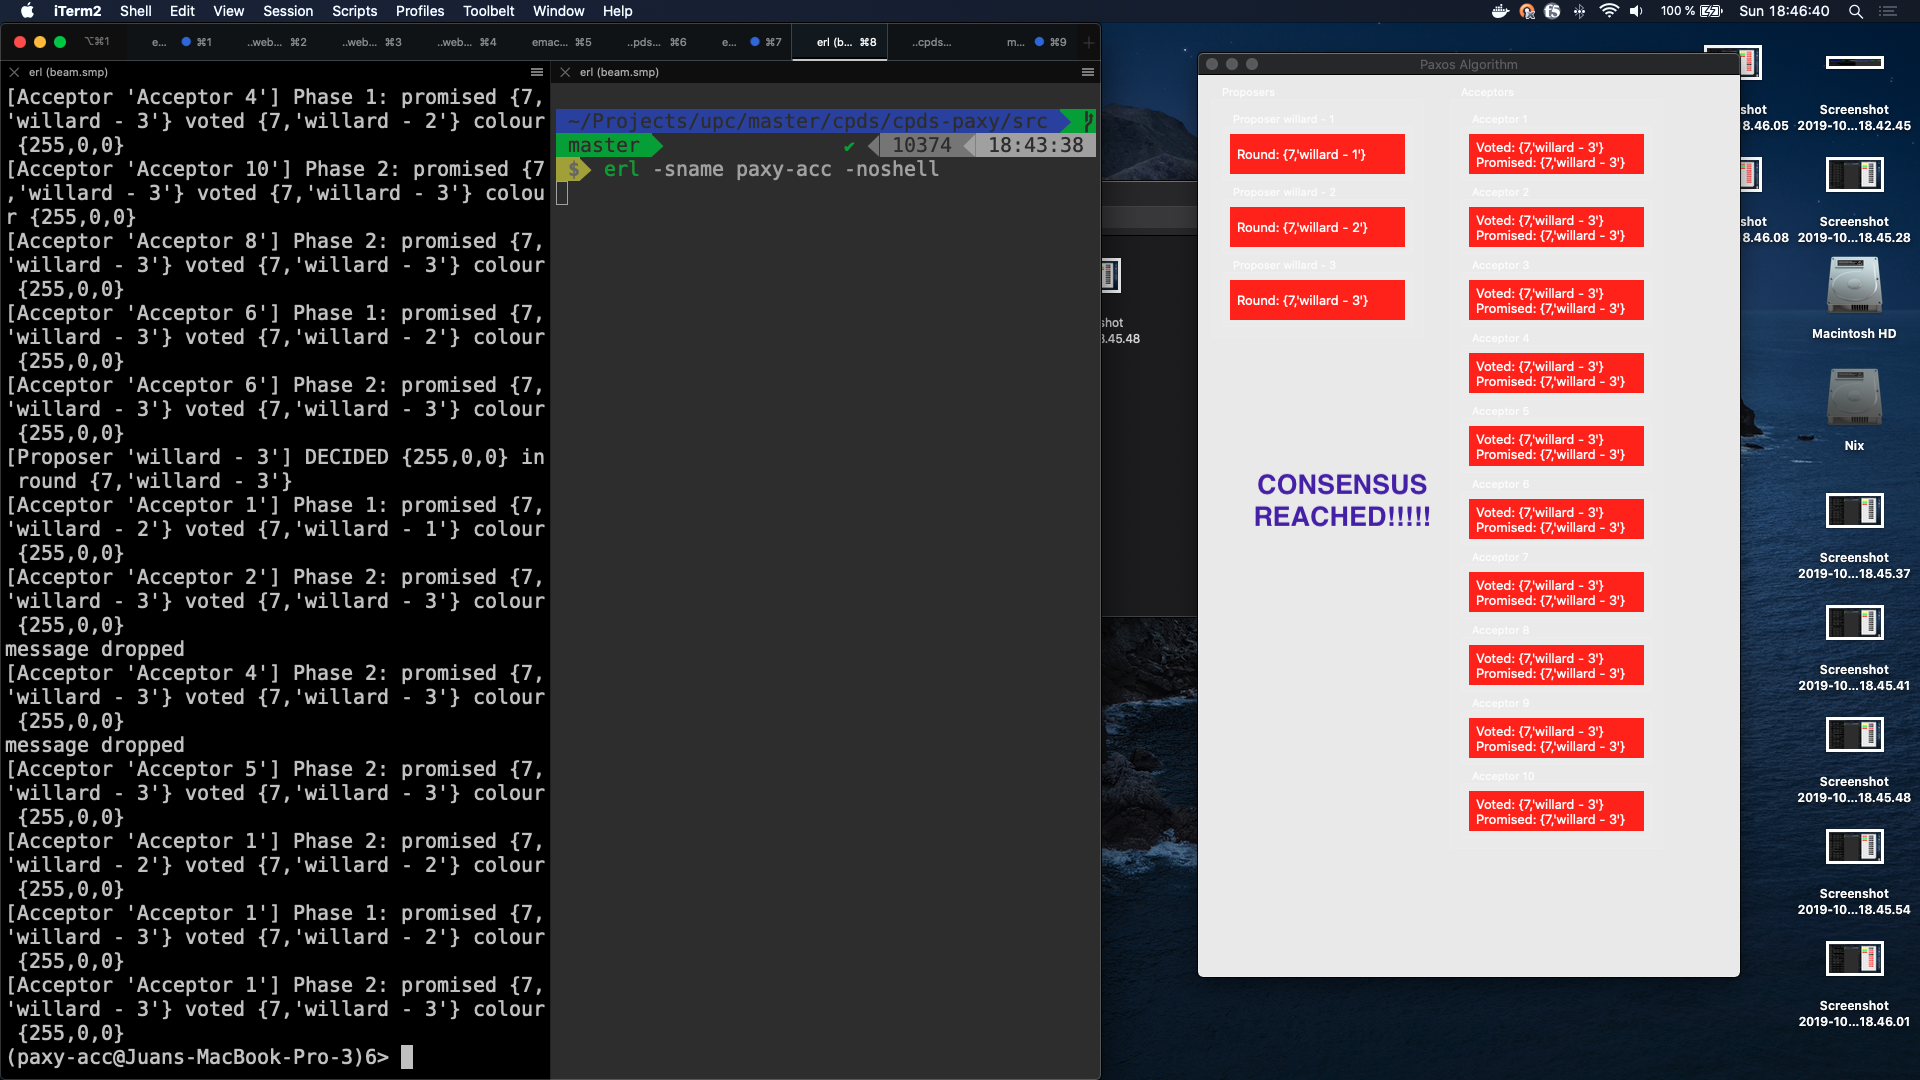
\includegraphics[width=\textwidth]{consensus}
  \captionof{figure}{Consensus Reached}
\end{minipage}\\

\subsection{Improvement based on sorry messages}
\subsubsection{Question}
Change the code of the collect/4 and vote/2 procedures to implement the aforementioned improvement and check how it works, especially whether it allows to get consensus faster.

\subsubsection{Answer}
We have successfully implemented the improvement on sorry messages. Now, if the number of sorry messages received is greater or equal to the number of Acceptors, the current round is skipped to avoid doing redundant work (it is not possible to reach a Quorum anymore in that round).\\

In the following Figure, we can see how an error is received and the Proposers increase the counter.\\
\begin{minipage}[t]{\linewidth}
  \centering
  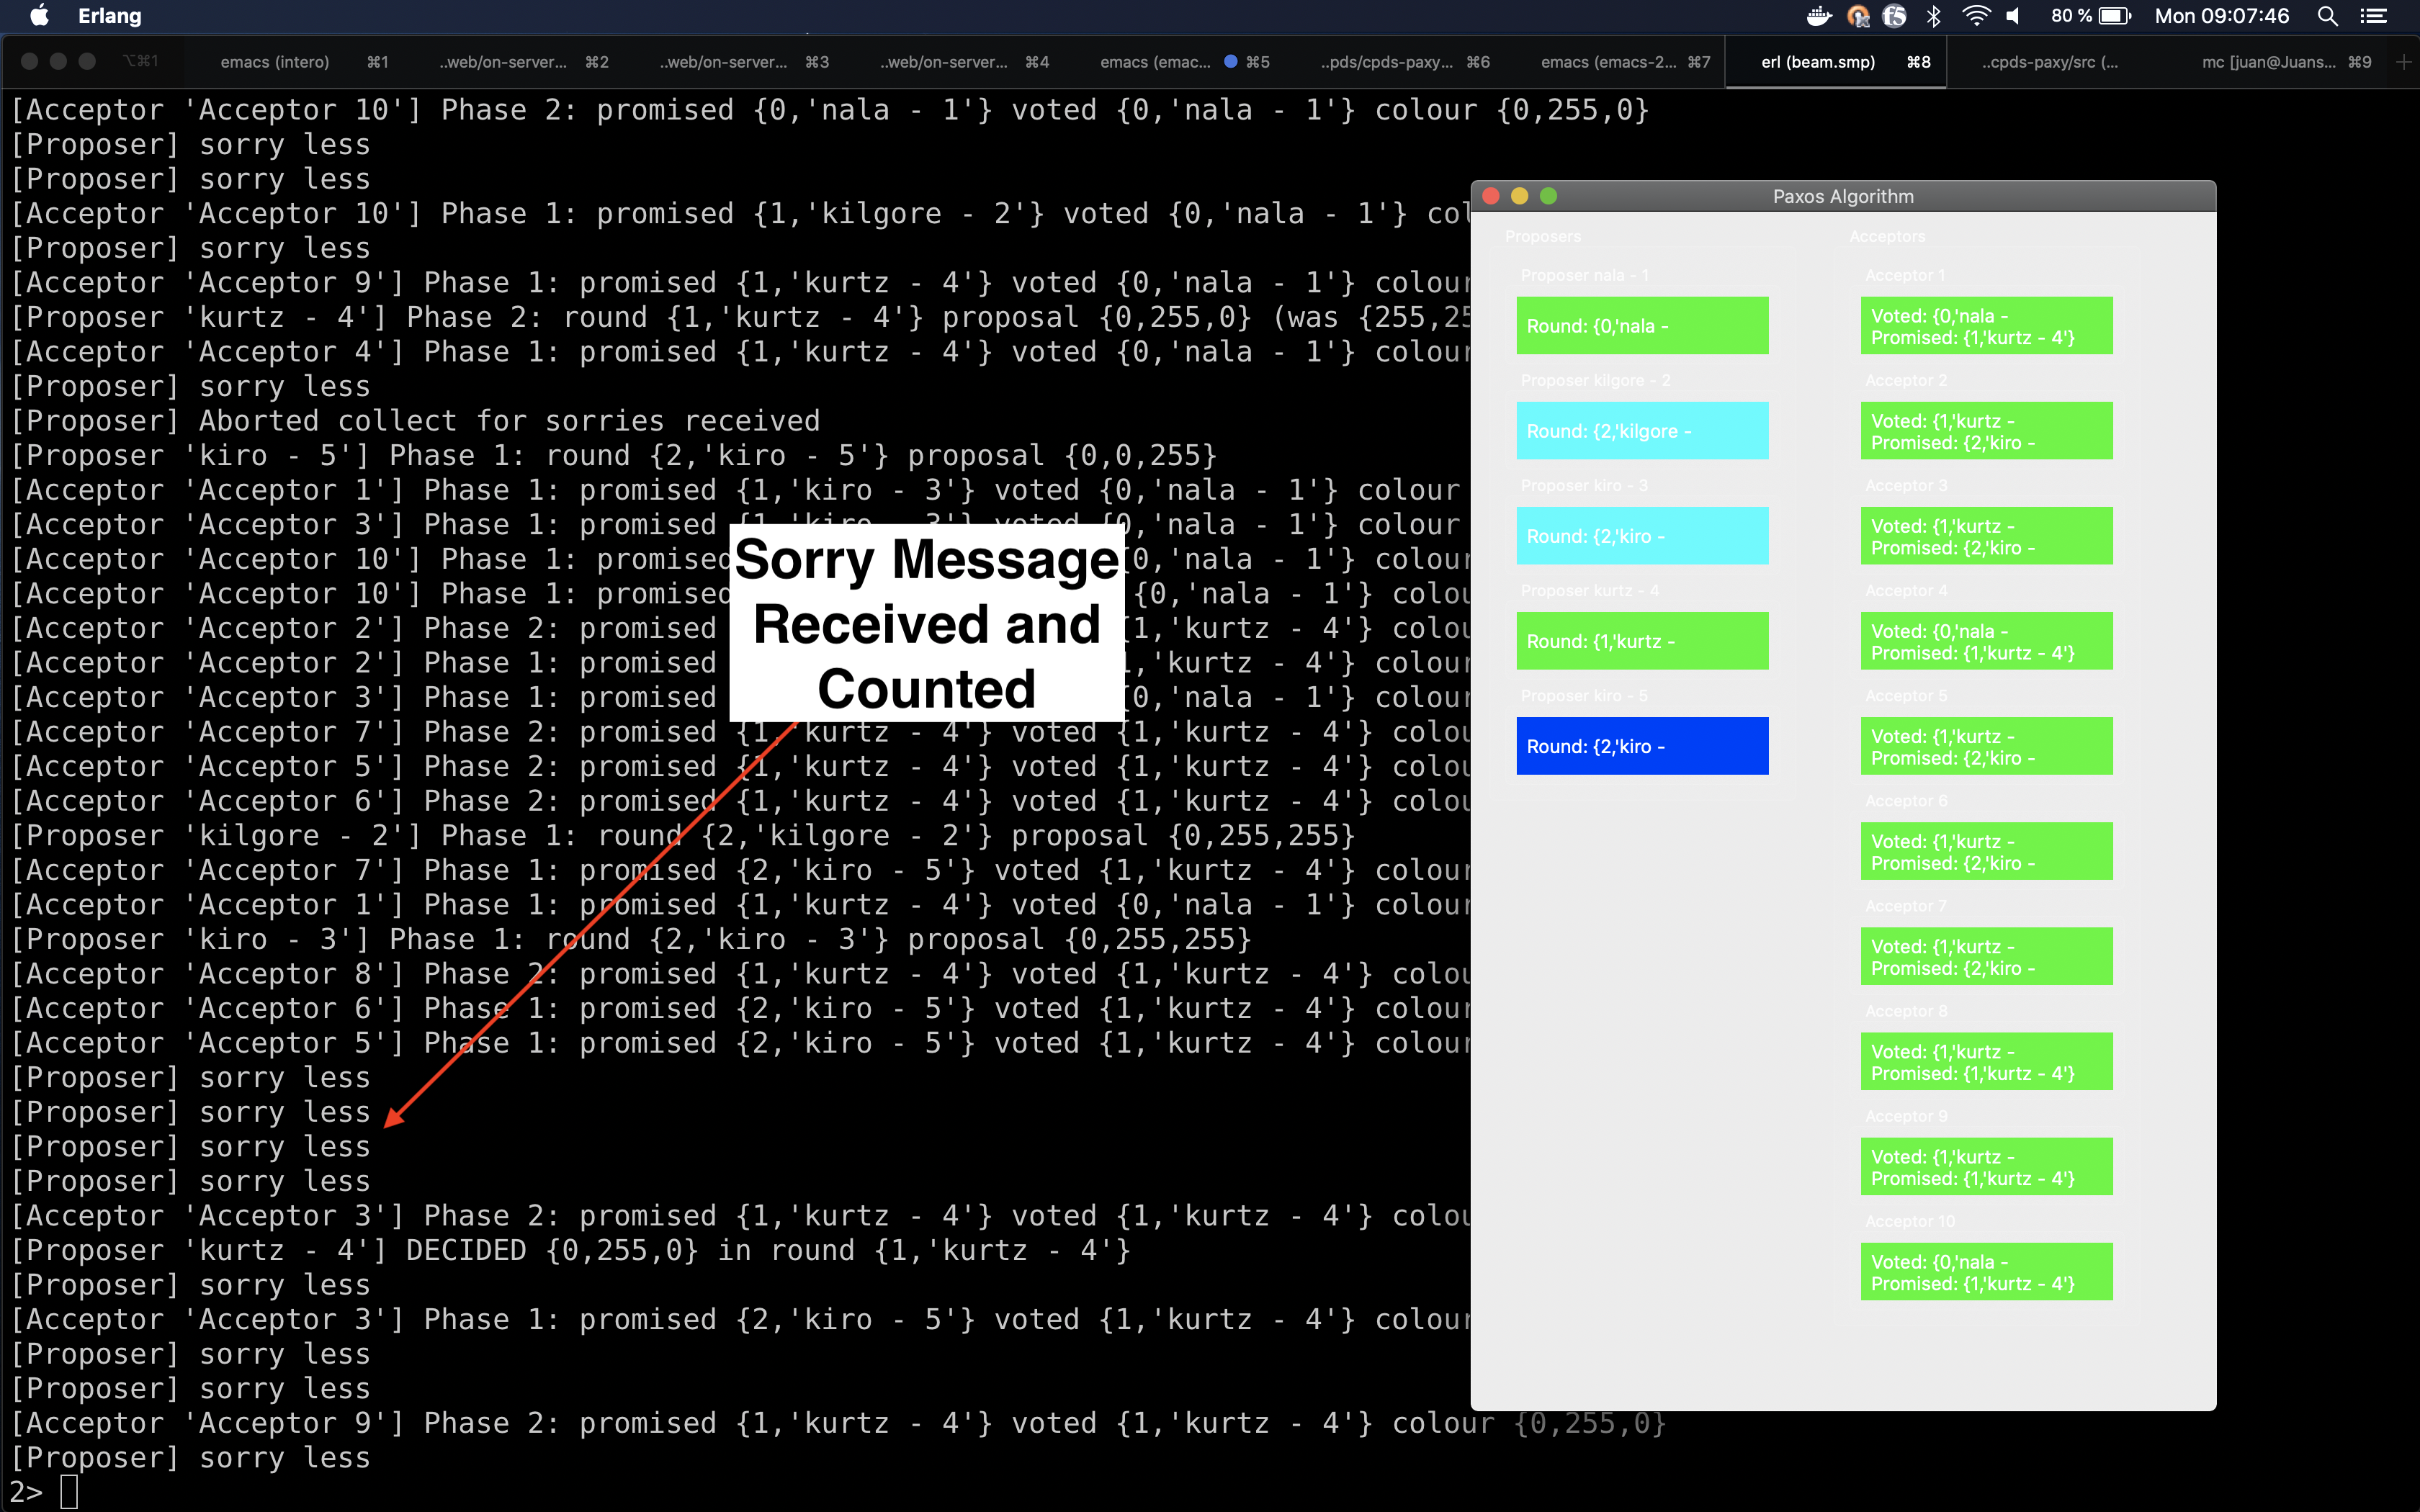
\includegraphics[width=\textwidth]{sorry_counted.png}
  \captionof{figure}{Sorry counted}
\end{minipage}\\\\

The next image shows how a round is aborted after receiving too many sorry messages.\\\\
\begin{minipage}[t]{\linewidth}
  \centering
  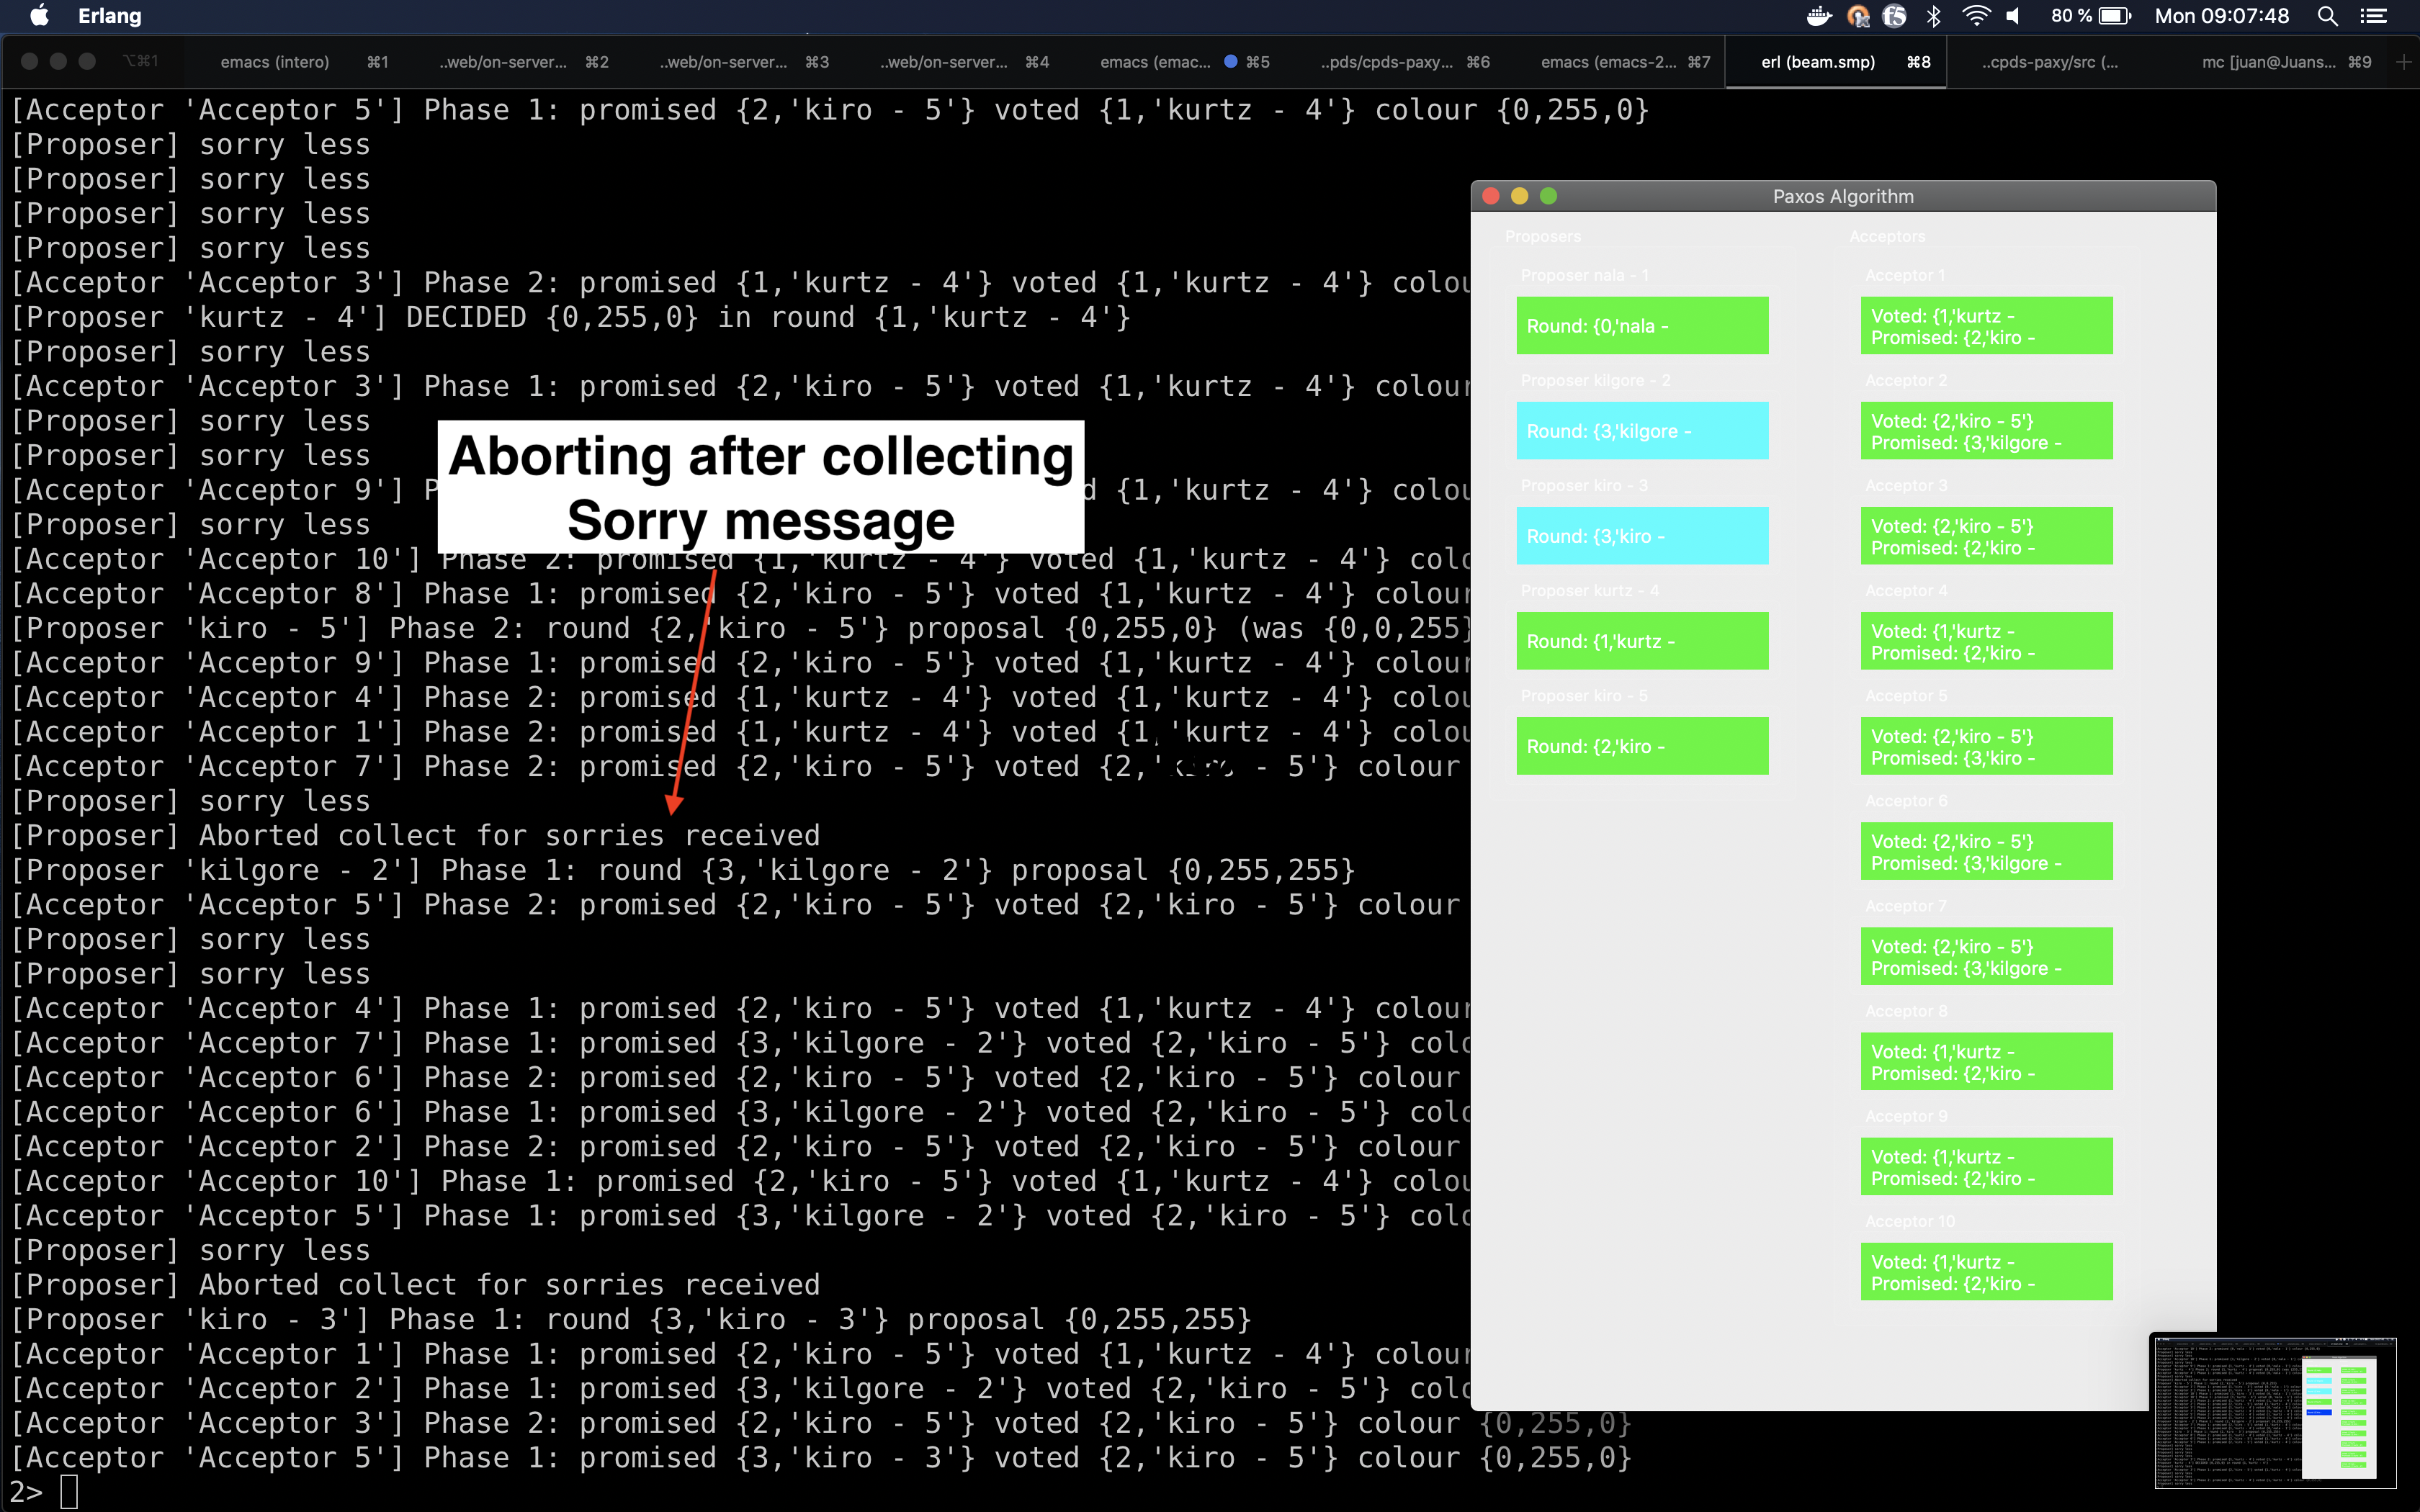
\includegraphics[width=\textwidth]{aborted_sorry.png}
  \captionof{figure}{Round aborted due sorry messages}
\end{minipage}\\\\

Finally, we show how the algorithm keeps running until a consensus is reached while skipping useless rounds. Therefore, improving the overall performance.\\\\
\begin{minipage}[t]{\linewidth}
  \centering
  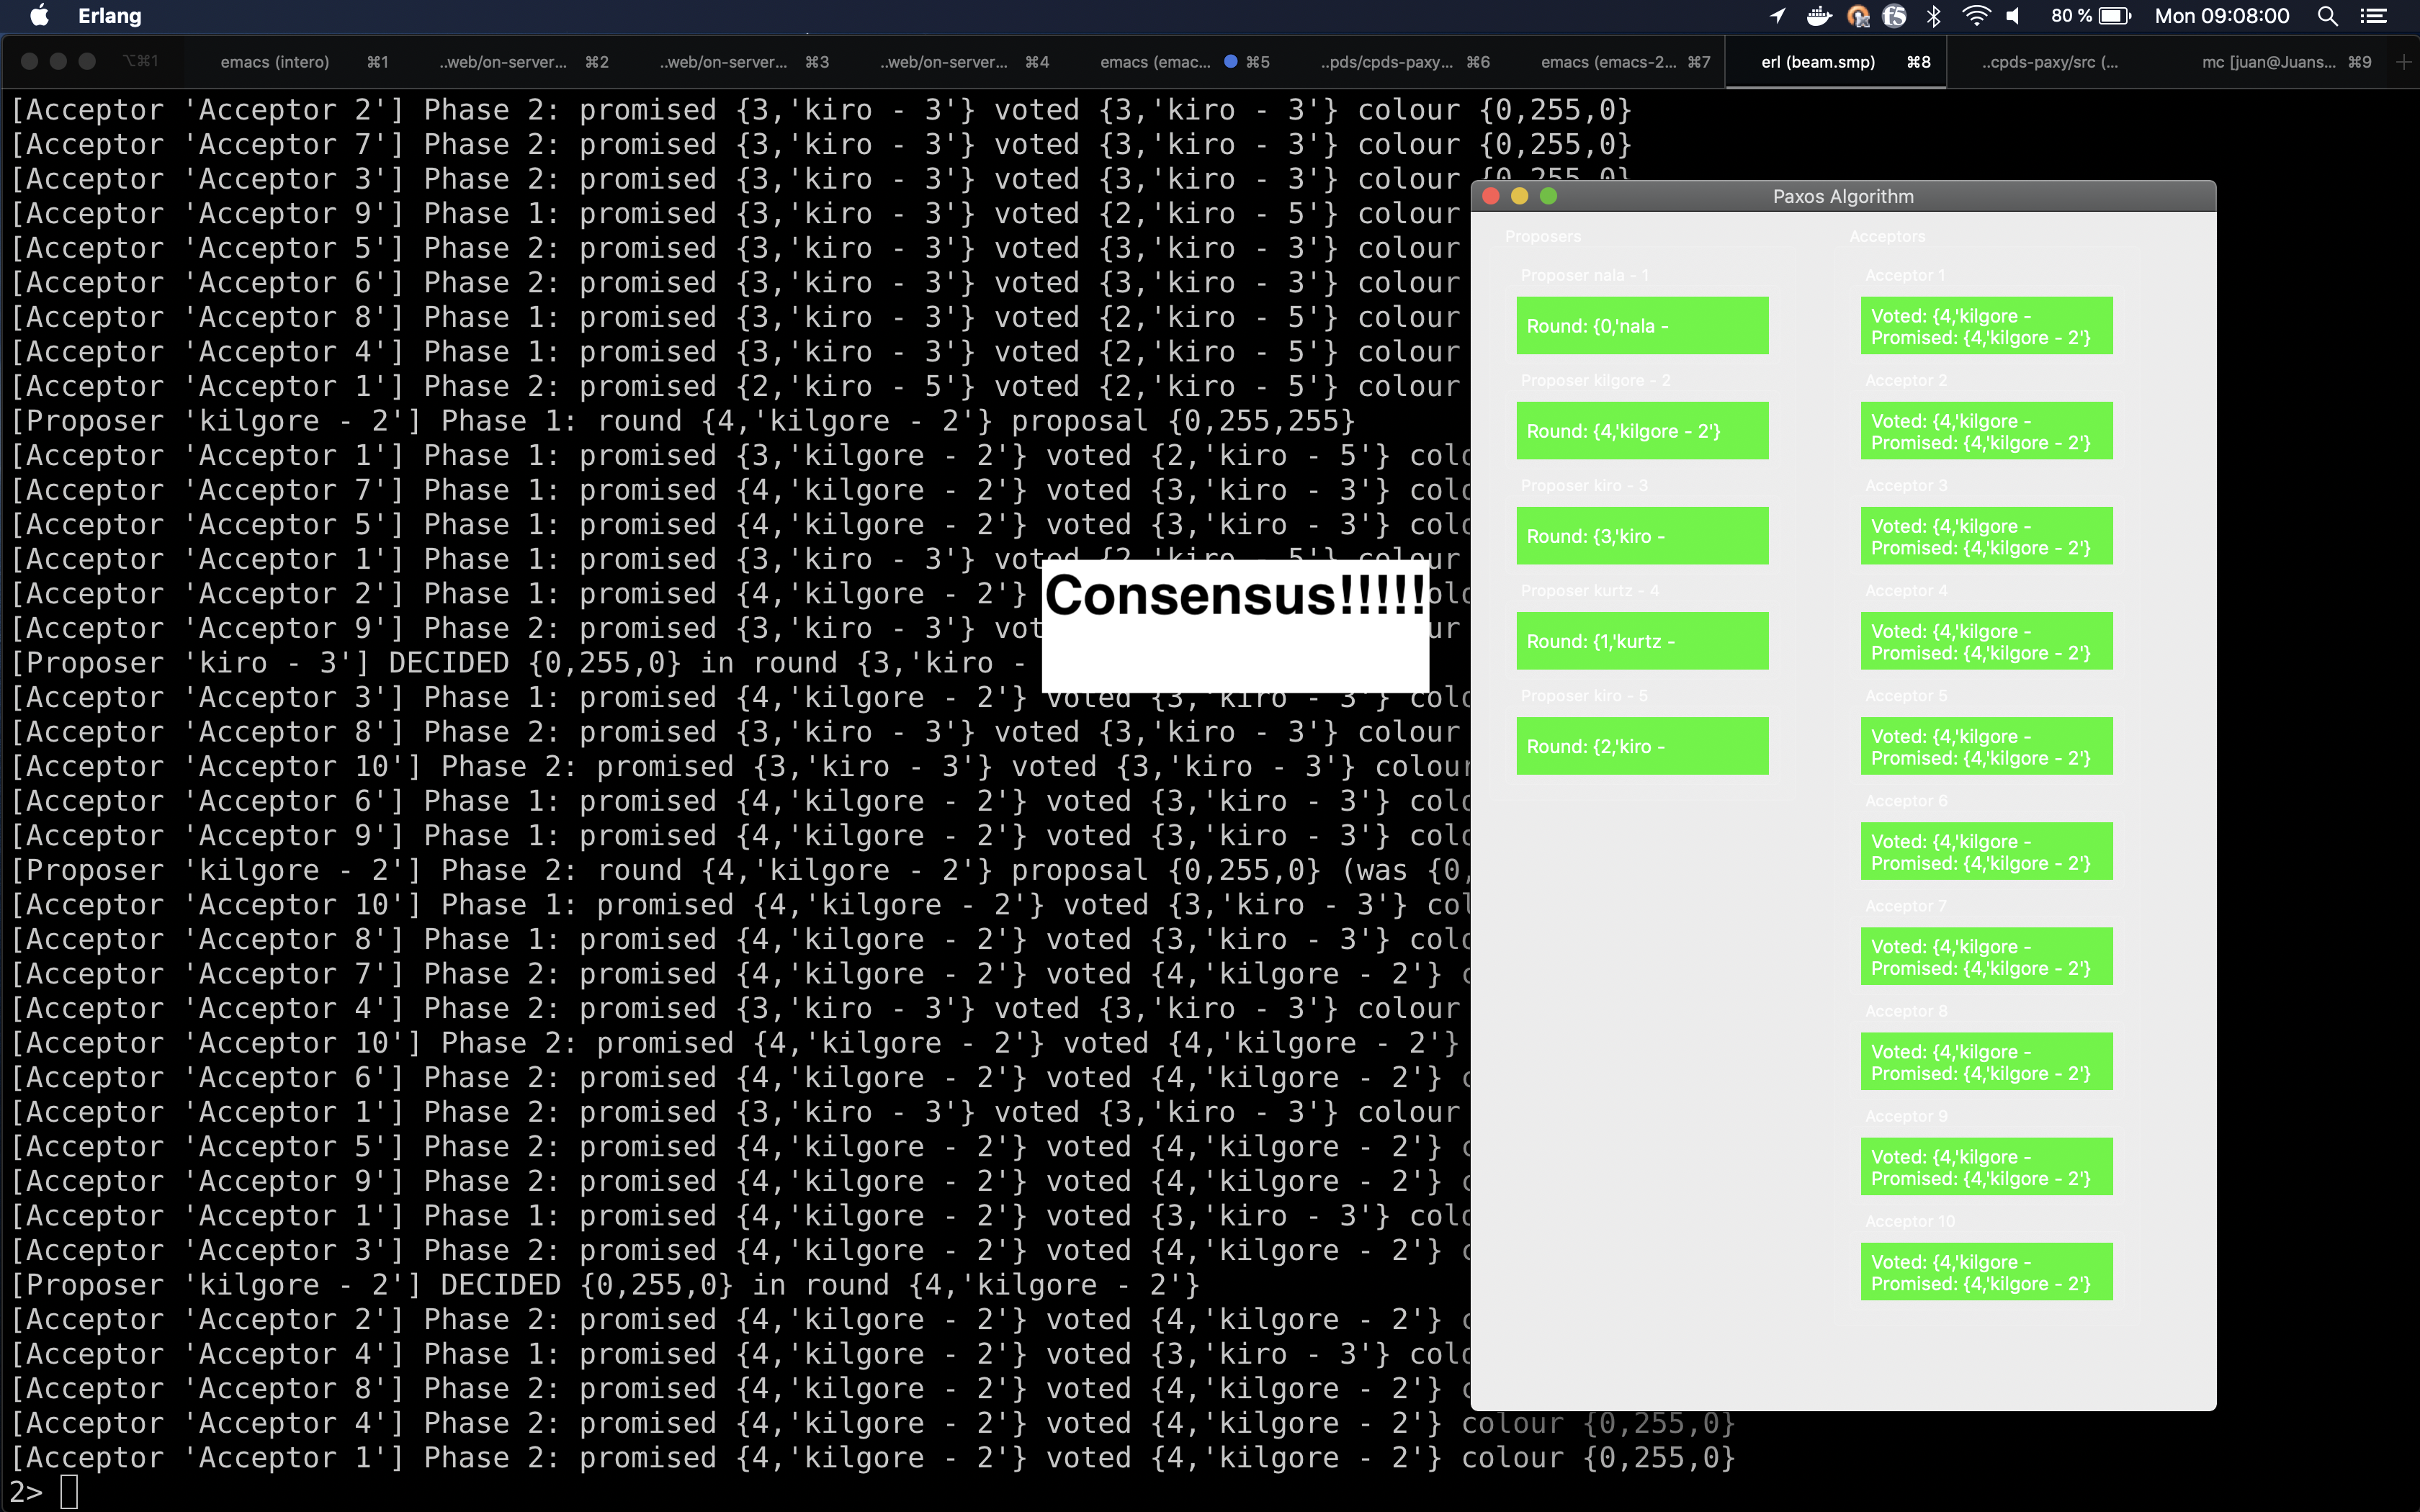
\includegraphics[width=\textwidth]{consensus_sorry.png}
  \captionof{figure}{Consensus reached after improved sorry method}
\end{minipage}\\

\section{Personal opinion}
After completing the algorithm, we all agree that it has been a good experience.
Not only we have worked on a real algorithm, but also it tries to solve an
important and intrinsic problem found in any distributed system, the global state (or the lack of it). What's more, we
have discovered Erlang, which can become a powerful tool in the future for us.
Still, the learning curve has bin a bit hard specially during the first
hours. Dedicating one or half a session showing and experiencing with a simple
test in Erlang may have helped. It has also been delightful to keep improving the algorithm with the fault tolerance and the implementation of the sorry messages.

\end{document}
